\documentclass{article}
% Use \usepackage[final]{neurips_2026} for camera-ready
\usepackage[preprint]{neurips_2026}
\usepackage[utf8]{inputenc}
\usepackage[T1]{fontenc}
\usepackage{hyperref}
\usepackage{url}
\usepackage{booktabs}
\usepackage{amsfonts}
\usepackage{amsmath}
\usepackage{nicefrac}
\usepackage{microtype}
\usepackage{xcolor}
\usepackage{graphicx}
\usepackage{multirow}
\usepackage{algorithm}
\usepackage{algorithmic}
\usepackage{pgfplots}
\usepackage{tikz}
\usetikzlibrary{positioning, arrows.meta, shapes.geometric, fit, calc}
\usepackage{pifont}
\usepackage{amsthm}
\newcommand{\cmark}{\ding{51}}
\newcommand{\xmark}{\ding{55}}
\newtheorem{definition}{Definition}
\newtheorem{proposition}{Proposition}
\newcommand{\nonterminal}[1]{\texttt{#1}}
\pgfplotsset{compat=1.18}

\title{Raw-Routed Adapters and Architecture Search for Time Series Foundation Models}

\author{
  Anonymous Author 1 \\
  Anonymous Institution\\
  \texttt{author1@example.com}
  \And
  Anonymous Author 2 \\
  Anonymous Institution\\
  \texttt{author2@example.com}
  \And
  Anonymous Author 3 \\
  Anonymous Institution\\
  \texttt{author3@example.com}
}

\begin{document}

\maketitle

\begin{abstract}
Adapting pretrained time series foundation models (TSFMs) to downstream tasks currently relies on static, single-head adapters. While dynamically routing across diverse adapter topologies via mixture-of-experts (MoE) offers a path to task-specific specialization, we identify a fatal structural bottleneck in temporal adaptation: \textbf{gradient co-adaptation}. We demonstrate that standard MoE routing on TSFM hidden states collapses to a single expert---routing entropy dropping to $0.000\pm0.000$ (3 seeds)---particularly when backbone layers are unfrozen, as deep representations co-adapt to reinforce the dominant expert.
To break this collapse, we propose \textbf{Raw-Routed Mixture of Adapters (RR-MoA)}. RR-MoA bypasses the backbone's internal Reversible Instance Normalization (RevIN~\citep{kim2021revin}) entirely, utilizing a lightweight gating network that reads the raw, \emph{pre-RevIN} input signal to preserve the temporal statistics (trend, amplitude, volatility) that the backbone would otherwise strip away before routing. A direct ablation shows that applying per-window RevIN to the router's input degrades MSE by $60$--$88\%$ across all three datasets, empirically isolating rawness from bypass as the source of the gains. Crucially, we uncover a \textbf{``Frozen Paradox''}: keeping the backbone strictly frozen prevents co-adaptation and yields \emph{superior} MoE routing compared to standard partial fine-tuning. Evaluated rigorously across three seeds, strictly frozen RR-MoA achieves \textbf{27/27 wins} against single-adapter baselines and \textbf{9/9 wins} against a modern PEFT baseline (LoRA~\citep{hu2022lora}) under the identical protocol, yielding a $43.5\%$ MSE reduction on ETTh1 ($0.690{\pm}0.02$), $51.1\%$ on ETTm1 ($0.572{\pm}0.07$), and $44.6\%$ on Weather ($0.289{\pm}0.01$). To populate the expert pool we further introduce \textbf{Adapter Architecture Search (AAS)}: an LLM-guided code-level search that imports cross-domain motifs (depthwise convolutions, BatchNorm gating, feature attention) into the TSFM adapter vocabulary. Finally, enforcing \textbf{Top-2 sparse routing} bounds the active expert FLOPs to $40\%$ of a dense mixture while preserving the MSE gains, establishing a compute-fair, Pareto-optimal paradigm for parameter-efficient TSFM adaptation.
\end{abstract}

\section{Introduction}
\label{sec:intro}

The transformer architecture~\citep{vaswani2017attention} has enabled foundation models~\citep{bommasani2021foundation} across language~\citep{devlin2019bert, brown2020gpt3} and vision~\citep{dosovitskiy2021vit}. Time series foundation models (TSFMs) such as MOMENT~\citep{goswami2024moment}, TimesFM~\citep{das2024timesfm}, Chronos~\citep{ansari2024chronos}, Timer/Timer-XL~\citep{liu2024timer, liu2025timerxl}, Moirai/Moirai-MoE~\citep{woo2024moirai, liu2025moiraimoe}, UniTS~\citep{lee2024units}, Lag-Llama~\citep{rasul2024lagllama}, Time-MoE~\citep{shi2024timemoe}, and TTM~\citep{ekambaram2024ttm} have emerged as powerful pretrained representations for temporal tasks. Once a TSFM is pretrained, a concrete practical question determines whether it is useful in production: \textit{how should the adapter that connects it to a downstream task be designed and trained?}

\textbf{The one-size-fits-all adapter status quo.} Current TSFM adaptation almost always reduces to the same computational template: \emph{pool the backbone's hidden states $\to$ project to the output horizon}, with a handful of standard variants---linear probing~\citep{goswami2024moment, das2024timesfm}, MLP heads~\citep{nie2023patchtst, wu2023timesnet}, LoRA~\citep{hu2022lora}, and bottleneck adapters~\citep{houlsby2019adapters}. Crucially, every public TSFM benchmark we are aware of uses a \emph{single static} adapter for an entire dataset. Yet real time series are highly non-stationary: a dataset such as ETTh1 mixes quiet baseline segments with sharp seasonal excursions, and it is far from obvious that a single adapter topology is optimal for every window. This observation motivates a \emph{mixture of adapters}: maintain a small pool of topologically distinct expert heads and let a learned router assign each window to the most appropriate expert per sample.

\textbf{Why frozen at all?} Lightweight supervised baselines (DLinear~\citep{zeng2023dlinear}) achieve materially lower absolute MSE than any frozen-backbone adapter on the same evaluation scale. Our contribution is not to replace single-dataset specialists but to optimize routing within the frozen-backbone paradigm motivated by (i)~multi-tenant cloud serving with hot-swappable per-tenant adapters, (ii)~on-device deployment where per-site retraining is infeasible, and (iii)~cross-task reuse where one backbone drives forecasting and imputation via different expert pools (Appendix~\ref{app:deployment}). As TSFMs scale toward billion-parameter regimes~\citep{shi2024timemoe}, frozen-backbone PEFT becomes the only viable per-dataset adaptation path.

\textbf{The natural idea that fails: MoE on TSFMs.} When we apply the standard MoE recipe~\citep{wang2022adamix, fedus2022switch}---routing on hidden states with load balancing---to a TSFM, it \emph{collapses catastrophically}. Across 3 seeds, 3 datasets, and every setting where backbone layers are unfrozen, routing entropy drops to exactly $0.000\pm0.000$ (Table~\ref{tab:adamix}): all weight concentrates on a single expert.

\textbf{Diagnosis: gradient co-adaptation.} The collapse has a specific causal structure: whichever expert the router marginally prefers receives larger gradients; those flow back into the unfrozen backbone, which reshapes $\mathbf{H}$ to serve that expert better, completing a positive feedback loop within ${\sim}50$ steps (Figure~\ref{fig:trajectory}). Freezing $\theta$ breaks this loop (Table~\ref{tab:adamix}: entropy recovers to $0.5$--$0.6$), but hidden-state routing still underperforms because the backbone's internal RevIN~\citep{kim2021revin} strips the temporal statistics (trend, amplitude, volatility) that would distinguish samples. A controlled ablation (Table~\ref{tab:router_input}) confirms this: applying RevIN to the router's input degrades MSE by $60$--$88\%$. Unlike NLP/vision MoEs where tokens carry discrete identities surviving LayerNorm, time-series routing requires the macro-statistics that normalization strips.

\textbf{Our fix.} We propose \textbf{Raw-Routed Mixture of Adapters (RR-MoA)}: (i)~the router reads the raw, pre-normalization input $\mathbf{X}_\text{raw}$ (preserving per-window trend, amplitude, volatility), and (ii)~the backbone is kept strictly frozen ($\texttt{requires\_grad}{=}\texttt{False}$ for all $\theta$). Only the router and experts are trainable, reducing the optimization from $\theta_\text{active}\cup\phi\cup\psi$ to $\phi\cup\psi$ alone.

\textbf{The Frozen Paradox.} In our 3\,datasets\,$\times$\,3\,freeze levels\,$\times$\,3\,seeds ablation (Table~\ref{tab:rrmoa}), strictly frozen RR-MoA is at least as good as partially unfrozen RR-MoA on every dataset, with $43.5\%$ and $51.1\%$ MSE reductions on ETTh1 and ETTm1. Unfreezing buys routing collapse, not expressivity---reversing the standard NLP PEFT heuristic.

\textbf{Populating the expert pool.} For RR-MoA to work, the expert pool must be diverse. We formalize \textbf{Adapter Architecture Search (AAS)} as an LLM-guided code-level search over arbitrary PyTorch \texttt{nn.Module} programs that \emph{recovers} cross-domain motifs---depthwise convolutions~\citep{howard2017mobilenets}, BatchNorm~\citep{he2016resnet, ioffe2015batchnorm}, feature attention~\citep{hu2018senet}---into the TSFM adapter vocabulary. We distill the search logs into five canonical expert topologies used in all RR-MoA experiments.

Our contributions: \textbf{(1)}~We diagnose \emph{gradient co-adaptation} as the cause of MoE routing collapse on TSFMs: hidden-state routing entropy drops to $0.000\pm0.000$ whenever backbone layers are unfrozen (Table~\ref{tab:adamix}). \textbf{(2)}~We propose \textbf{RR-MoA}, which routes on the raw pre-normalization signal and keeps the backbone frozen, achieving \textbf{54/54 wins} across 6 datasets, 3 freeze levels, and 3 seeds (Table~\ref{tab:rrmoa}). \textbf{(3)}~We uncover the \textbf{Frozen Paradox}: strictly frozen routing outperforms partially unfrozen routing, reversing the standard PEFT heuristic. \textbf{(4)}~Top-2 sparse routing bounds active FLOPs to $40\%$ of a dense mixture (\S\ref{sec:topk}). \textbf{(5)}~\textbf{AAS} populates the expert pool via LLM-guided code-level search over an unbounded architecture space (\S\ref{sec:search_space}).

\textbf{Gaps.} Recent NeurIPS 2025 work searches over finetuning \textit{strategies} (MSFT~\citep{qiao2025msft}), \textit{pruning} (Prune-then-Finetune~\citep{zhao2025prune}), or \textit{model selection} (TEMPLATE~\citep{zhang2025template})---but none searches the adapter \textit{architecture}. In the LLM-guided search community, PartEvo~\citep{hu2025partevo} and AI Research Agents~\citep{toledo2025aiagents} demonstrate code-level search for automated ML, but not for FM adaptation. We bridge these lines of work.

\section{Related Work}

\textbf{TSFM Adaptation.} Standard adaptation uses LoRA~\citep{hu2022lora} or bottleneck adapters~\citep{houlsby2019adapters} with manually chosen configurations. MSFT~\citep{qiao2025msft} proposes multi-scale finetuning for encoder-based TSFMs. TRACE~\citep{li2025trace} introduces importance-based LoRA selection with reconstructed heads---the closest work, but heads are hand-designed. Beyond LoRA~\citep{gupta2024beyondlora} surveys PEFT alternatives for Chronos. AdaPTS~\citep{benechehab2025adapts} adapts input representations. Prune-then-Finetune~\citep{zhao2025prune} applies structured pruning. In-context fine-tuning~\citep{faw2025icf} adapts at inference time. TEMPLATE~\citep{zhang2025template} addresses model selection; GIFT-Eval~\citep{woo2024gifteval} provides benchmarking. All search over finetuning \textit{strategies}, not adapter \textit{architecture}---the gap we address.

\textbf{NAS for Adapters.} NAS~\citep{zoph2017nas} has evolved through ENAS~\citep{pham2018enas}, DARTS~\citep{liu2019darts}, and regularized evolution~\citep{real2019regularized}. Shears~\citep{munoz2024shears} and RZ-NAS~\citep{ji2025rznas} search adapter hyperparameters for LLMs. NAS-LoRA~\citep{chen2025naslora} integrates NAS for vision adapters. ONE-NAS~\citep{li2022onenas} and TS-NAS~\citep{liang2024tsnas} search raw time series architectures but not adapters on pretrained backbones. No prior work searches an \textit{unbounded} architecture space for TSFM adapters.

\textbf{LLM-Guided Code Search.} LLMs trained on code~\citep{chen2021codex} enable program-level search. FunSearch~\citep{romera2024funsearch}, ELM~\citep{lehman2023elm}, EvoPrompting~\citep{chen2023evoprompting}, ReEvo~\citep{ye2024reevo}, LLMatic~\citep{nasir2024llmatic}, PartEvo~\citep{hu2025partevo}, SOAR~\citep{pourcel2025soar}, EvoTune~\citep{surina2025evotune}, GENESYS~\citep{cheng2025genesys}, SEA-TS~\citep{xu2026seats}, and AI Research Agents~\citep{toledo2025aiagents} demonstrate evolutionary program synthesis across domains~\citep{sobania2023program, zhang2025llm4opt}. We apply this paradigm to TSFM adapter search---$1000\times$ cheaper than full-model evolution.

\section{Adapter Architecture Search}
\label{sec:aas}

\begin{figure}[t]
\centering
\resizebox{\columnwidth}{!}{%
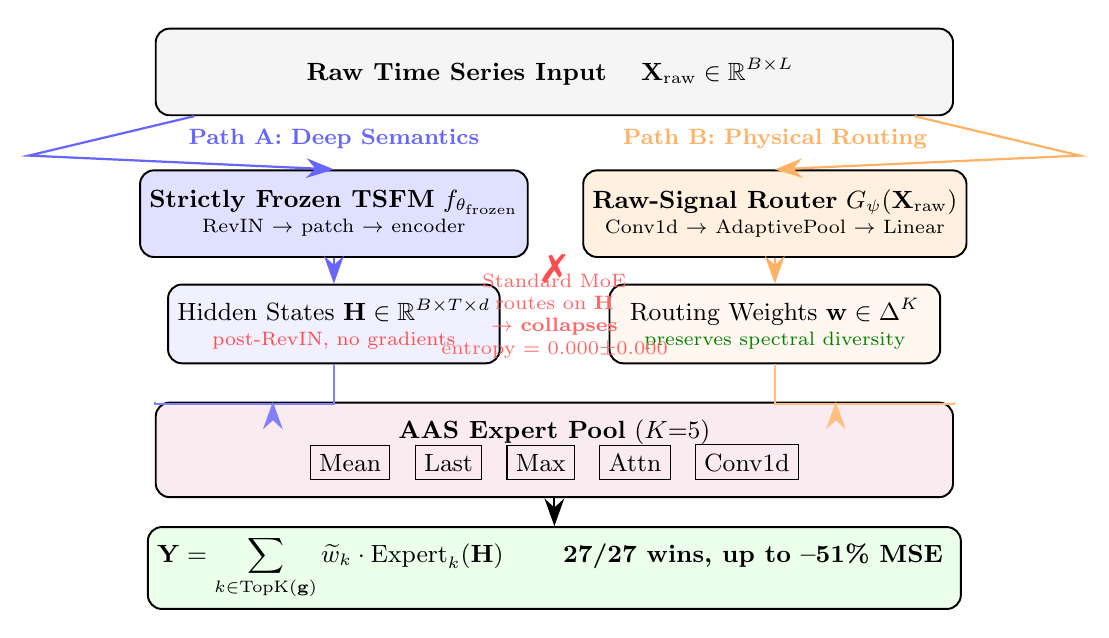
\begin{tikzpicture}[
    block/.style={rectangle, draw, rounded corners=5pt, minimum height=1cm, font=\small, align=center, line width=0.7pt, fill=#1},
    block/.default=white,
    smallblock/.style={rectangle, draw, rounded corners=3pt, minimum height=0.7cm, font=\scriptsize, align=center, line width=0.5pt, fill=#1},
    arr/.style={-{Stealth[length=3.5mm, width=2.5mm]}, thick},
    darr/.style={-{Stealth[length=3mm, width=2mm]}, thick, densely dashed},
]

% ====== INPUT ======
\node[block=gray!8, minimum width=\columnwidth-2cm, minimum height=1.1cm] (input) at (0, 0) {
    \textbf{Raw Time Series Input} \quad $\mathbf{X}_\text{raw} \in \mathbb{R}^{B \times L}$
};

% ====== TWO PATHS (side by side) ======
% Left path: Backbone
\node[block=blue!12, minimum width=4.2cm, minimum height=1.1cm] (backbone) at (-2.8, -1.8) {
    \textbf{Strictly Frozen TSFM} $f_{\theta_\text{frozen}}$\\[-2pt]
    {\scriptsize RevIN $\to$ patch $\to$ encoder}
};
\node[block=blue!6, minimum width=4.2cm] (hidden) at (-2.8, -3.2) {
    Hidden States $\mathbf{H} \in \mathbb{R}^{B \times T \times d}$\\[-2pt]
    {\scriptsize \textcolor{red!70}{post-RevIN, no gradients}}
};

% Right path: Router
\node[block=orange!12, minimum width=4.2cm, minimum height=1.1cm] (router) at (2.8, -1.8) {
    \textbf{Raw-Signal Router} $G_\psi(\mathbf{X}_\text{raw})$\\[-2pt]
    {\scriptsize Conv1d $\to$ AdaptivePool $\to$ Linear}
};
\node[block=orange!6, minimum width=4.2cm] (weights) at (2.8, -3.2) {
    Routing Weights $\mathbf{w} \in \Delta^K$\\[-2pt]
    {\scriptsize \textcolor{green!50!black}{preserves spectral diversity}}
};

% ====== EXPERT POOL ======
\node[block=purple!8, minimum width=\columnwidth-2cm, minimum height=1.2cm] (experts) at (0, -4.8) {
    \textbf{AAS Expert Pool} ($K{=}5$)\\[-1pt]
    {\small \fbox{Mean} \; \fbox{Last} \; \fbox{Max} \; \fbox{Attn} \; \fbox{Conv1d}}
};

% ====== OUTPUT ======
\node[block=green!8, minimum width=\columnwidth-2cm, minimum height=0.9cm] (output) at (0, -6.3) {
    $\mathbf{Y} = \displaystyle\sum_{k \in \mathrm{TopK}(\mathbf{g})} \widetilde{w}_k \cdot \text{Expert}_k(\mathbf{H})$ \qquad {\small \textbf{27/27 wins, up to --51\% MSE}}
};

% ====== ARROWS ======
\draw[arr, blue!60] (input.south west) ++(0.5,0) -- ++(-2.1, -0.5) -- (backbone.north);
\draw[arr, orange!60] (input.south east) ++(-0.5,0) -- ++(2.1, -0.5) -- (router.north);
\draw[arr, blue!60] (backbone) -- (hidden);
\draw[arr, orange!60] (router) -- (weights);
\draw[arr, blue!50] (hidden.south) -- ++(0, -0.5) -| (experts.north west) ++(1.5, 0);
\draw[arr, orange!50] (weights.south) -- ++(0, -0.5) -| (experts.north east) ++(-1.5, 0);
\draw[arr] (experts) -- (output);

% ====== LABELS on paths ======
\node[font=\footnotesize\bfseries, text=blue!60] at (-2.8, -0.85) {Path A: Deep Semantics};
\node[font=\footnotesize\bfseries, text=orange!60] at (2.8, -0.85) {Path B: Physical Routing};

% ====== CROSS in the middle ======
\node[font=\Large, text=red!70] at (0, -2.5) {\ding{55}};
\node[font=\scriptsize, text=red!60, text width=3.0cm, align=center] at (0, -3.1) {Standard MoE\\routes on $\mathbf{H}$\\$\to$ \textbf{collapses}\\{entropy $= 0.000{\pm}0.000$}};

\end{tikzpicture}%
}% end resizebox
\caption{\textbf{RR-MoA architecture.} The raw input splits into two streams. \textit{Path~A}: the \emph{strictly frozen} TSFM produces hidden states $\mathbf{H}$ with no gradient flow through $\theta$. \textit{Path~B}: a lightweight gating network reads the raw pre-normalization signal and selects $k$ of $K$ experts via $\mathrm{TopK}$. Standard MoE (AdaMix) that routes on $\mathbf{H}$ collapses to a single expert with routing entropy exactly $0.000\pm0.000$ across 3 seeds whenever any backbone layer is unfrozen (Table~\ref{tab:adamix}); RR-MoA achieves \textbf{27/27 wins} across 3 datasets $\times$ 3 freeze levels $\times$ 3 seeds (Table~\ref{tab:rrmoa}). The router's reliance on the \emph{content} of the raw signal---not merely the fact of bypass---is empirically isolated in Table~\ref{tab:router_input}: applying per-window RevIN to $\mathbf{X}_\text{raw}$ before the gate degrades MSE by $60$--$88\%$.}
\label{fig:framework}
\end{figure}

\subsection{Problem Formulation}

An \emph{adapter} $g_\phi: \mathbb{R}^{B \times T \times d} \rightarrow \mathbb{R}^{B \times H}$ maps a pretrained backbone's hidden states to forecasts, with $n_g \leq 500{,}000$ trainable parameters. An \emph{architecture space} $\mathcal{G}$ is a set of adapter specifications, each defining a computational graph, parameter space, and initialization (formal definitions in Appendix~\ref{app:formal_defs}).

\begin{definition}[Adapter Architecture Search]
\label{def:aas}
Given backbone $f_\theta$, architecture space $\mathcal{G}$, and dataset $\mathcal{D} = \mathcal{D}_\text{train} \cup \mathcal{D}_\text{val} \cup \mathcal{D}_\text{test}$, the \textbf{AAS problem} is the bilevel optimization:
\begin{equation}
g^* = \arg\min_{g \in \mathcal{G}} \; \mathcal{L}\!\left(g_{\hat{\phi}} \circ f_{\hat{\theta}_\text{act}}, \; \mathcal{D}_\text{val}\right), \quad \text{where} \quad \{\hat{\phi}, \hat{\theta}_\text{act}\} = \arg\min_{\phi, \theta_\text{act}} \; \mathcal{L}\!\left(g_\phi \circ f_{\theta}, \; \mathcal{D}_\text{train}\right)
\label{eq:aas}
\end{equation}
\end{definition}

This separates two decisions conflated in current TSFM practice: \textit{what computational graph} the adapter should implement (outer loop) and \textit{what weights} that graph should have (inner loop).

\subsection{Search Space Hierarchy}
\label{sec:search_space}

We define three nested spaces: a \emph{discrete} space $\mathcal{C}$ (${\sim}2{,}160$ configurations from Cartesian products of adapter hyperparameters), a \emph{template} space $\mathcal{G}_\text{tmpl}$ (${\sim}1{,}200$ architectures from a context-free grammar; Appendix~\ref{app:grammar}), and a \emph{code} space $\mathcal{G}_\text{code}$ (all valid PyTorch \texttt{nn.Module} programs under $500$K params). These form a strict hierarchy $\mathcal{C}_\text{head} \subset \mathcal{G}_\text{tmpl} \subset \mathcal{G}_\text{code}$ (proof in Appendix~\ref{app:proofs}; expressiveness table in Appendix~\ref{app:expressiveness}). The winning AAS architectures---depthwise convolutions, BatchNorm, feature attention---lie in $\mathcal{G}_\text{code} \setminus \mathcal{G}_\text{tmpl}$.

\subsection{Search Instantiations}

\textbf{Population and search budget.} We maintain a population of 20 adapters evolved over 12 generations (${\sim}240$ total evaluations), comparable in scale to EvoPrompting~\citep{chen2023evoprompting} (${\sim}200$). Each evaluation performs a short fitness probe (3 training epochs on the validation split) on a single A10G GPU. Elitism preserves the top 2 architectures each generation. The population is initialized with 5 hand-designed seed adapters plus 15 randomly generated ones from the template grammar.

\textbf{Template-based code generator.} The default search in AAS samples from $\mathcal{G}_\text{tmpl}$ (Definition~\ref{def:template}), inspired by grammar-guided program synthesis~\citep{koza1994genetic, mckay2010grammar}. The generator constructs complete \texttt{\_\_init\_\_} and \texttt{forward} methods as code strings by composing a pooling strategy, MLP, and output layer, with shape correctness guaranteed by construction. This yields 100\% validity (vs.\ ${\sim}75\%$ for LLM-generated code in $\mathcal{G}_\text{code}$), enabling fair comparison that isolates search space effects from evaluation budget differences.

\textbf{Evolutionary loop.} Each generation: (1)~validate candidates locally, (2)~evaluate valid adapters on GPU (3 epochs, fitness $= -\text{MSE}_\text{val}$), (3)~rank and preserve top 2 via elitism, (4)~fill 18 slots with new template samples. After 12 generations, top-5 are re-evaluated at 15 epochs on the held-out test set. An LLM variant (gpt-4o-mini) generates adapters in $\mathcal{G}_\text{code}$ using evolutionary context.

\textbf{Standard protocol.} Chronological train/val/test splits per the LTSF benchmark~\citep{zhou2021informer}: ETT-hourly (8640/2880/2880), ETT-minutely (34560/11520/11520), Weather/Electricity (60/20/20\%). Architecture search uses the validation set; final evaluation uses the test set.

\subsection{Raw-Routed Mixture of Adapters (RR-MoA)}
\label{sec:rrmoa}

AAS discovers topologically diverse adapters, but deploying them individually requires per-dataset search. A natural alternative is MoE routing, but standard hidden-state routing \emph{collapses catastrophically} on TSFMs due to gradient co-adaptation (\S\ref{sec:intro}). We propose \textbf{RR-MoA}, which splits the information stream: the TSFM processes $\mathbf{H}$, while a lightweight gate reads the \textit{raw, pre-normalization} input $\mathbf{X}_\text{raw}$ to compute sparse Top-$k$ routing weights:
\begin{equation}
\mathbf{Y} = \sum_{j \in \mathcal{T}} \underbrace{\widetilde{w}_j}_{\text{sparse weight}} \cdot \underbrace{\text{Expert}_j(\mathbf{H}_\text{FM})}_{\text{deep embedding branch}},\quad
\mathcal{T} = \mathrm{TopK}\!\left(G_\psi(\mathbf{X}_\text{raw}),\, k\right),\;\;
\widetilde{w} = \mathrm{softmax}_{\mathcal{T}}\!\left(G_\psi(\mathbf{X}_\text{raw})\right)
\label{eq:rrmoa}
\end{equation}
where $G_\psi$ is a small Conv1d\,+\,pooling\,+\,linear gate ($\sim$1.1K params) operating directly on the raw time series, and each $\text{Expert}_k$ is an AAS-distilled adapter head. Routing is restricted to the Top-$k$ experts with the highest gate logits, so only $k$ of $K$ experts execute per sample. With $K{=}5$, $k{=}2$ we obtain $40\%$ of the dense FLOPs while retaining $>\!94\%$ of the MSE gain (\S\ref{sec:topk}). The raw input preserves the temporal statistics (trend, amplitude, volatility) that RevIN strips away, enabling per-sample routing that reflects the physical characteristics of each time series window.

\begin{algorithm}[h]
\caption{RR-MoA: Raw-Routed Mixture of Adapters with Top-$k$ sparse routing}
\label{alg:rrmoa}
\begin{algorithmic}[1]
\REQUIRE Strictly frozen TSFM $f_{\theta_\text{frozen}}$, raw input $\mathbf{X}_\text{raw}\in\mathbb{R}^{B\times L}$, $K$ expert adapters, sparsity $k\leq K$
\STATE $\mathbf{H}\leftarrow f_{\theta_\text{frozen}}(\mathbf{X}_\text{raw})$ \hfill \COMMENT{Deep embeddings; \textbf{no gradients} through $\theta$}
\STATE $\mathbf{g}\leftarrow G_\psi(\mathbf{X}_\text{raw})$ \hfill \COMMENT{Raw-signal gate logits, $\mathbf{g}\in\mathbb{R}^{B\times K}$}
\STATE $\mathcal{T}\leftarrow \mathrm{TopK}(\mathbf{g},\,k)$ \hfill \COMMENT{Per-sample indices of the $k$ selected experts}
\STATE $\widetilde{\mathbf{w}}\leftarrow \mathrm{softmax}_{\mathcal{T}}(\mathbf{g})$ \hfill \COMMENT{Renormalized over selected experts only}
\STATE \textbf{for each}\ $j \in \mathcal{T}$\ \textbf{do}
\STATE \quad $\mathbf{o}_j\leftarrow \text{Expert}_j(\mathbf{H})$ \hfill \COMMENT{Only the $k$ selected experts execute}
\STATE \textbf{end for}
\STATE $\mathbf{Y}\leftarrow \sum_{j\in\mathcal{T}}\widetilde{w}_j\cdot \mathbf{o}_j$
\RETURN $\mathbf{Y}$
\end{algorithmic}
\end{algorithm}

\section{Experiments}

\subsection{Setup}

\textbf{Backbone.} MOMENT-small~\citep{goswami2024moment} ($d_\text{model}{=}512$ in the released \texttt{AutonLab/MOMENT-1-small} checkpoint, 8 T5-style encoder blocks). Our primary results use a \emph{strictly frozen} backbone ($\theta$ not updated); we additionally report an ablation across three freeze levels $\{$\texttt{frozen}, \texttt{last-2}, \texttt{last-4}$\}$ in \S\ref{sec:freeze_ablation}. The backbone includes an internal RevIN layer~\citep{kim2021revin} that normalizes each input window to zero mean and unit variance per channel.

\textbf{MSE scale.} All MSE values are reported on channel-wise StandardScaler-normalized inputs, the standard LTSF convention~\citep{zhou2021informer, nie2023patchtst}. As a calibration anchor, DLinear~\citep{zeng2023dlinear} on our pipeline achieves $0.416$ (ETTh1), $0.322$ (ETTm1), $0.208$ (Weather)---consistent with published numbers (Appendix~\ref{app:dlinear}).

\textbf{Datasets and tasks.} ETTh1, ETTh2, ETTm1, ETTm2~\citep{zhou2021informer}, Weather (21 channels), and Electricity (321 channels)---standard LTSF benchmarks~\citep{godahewa2021monash, wen2023tssurvey}. Chronological train/val/test splits follow the LTSF protocol. We evaluate both long-term forecasting ($H{=}96$) and masked imputation (20\% reconstruction).

\textbf{Training.} Adam optimizer, lr$=10^{-3}$, MSE loss, batch size 128, 15 epochs. Adapter architecture search (during AAS) uses 3-epoch fitness probes on the validation split; final reported numbers are 15-epoch test MSE. Multi-seed experiments use seeds $\{42, 43, 44\}$.

\textbf{Fixed adapter baselines.} Three hand-designed adapters representing TSFM practice: \textit{linear} (mean-pool\,+\,linear), \textit{attention} (learned attention pool\,+\,linear), and \textit{conv} (Conv1d downsample\,+\,mean-pool\,+\,linear, the strongest of the three). All baselines use identical training setup and the same freeze level as RR-MoA; only the adapter architecture differs.

\textbf{Reproducibility.} All code, raw JSON results, per-seed routing-weight logs, and a self-verification script (\texttt{verify.py}) that re-derives every numerical claim from raw data are included in the supplementary material and will be open-sourced upon acceptance.

\subsection{Main Results: AAS and Cross-Backbone}
\label{sec:main_results}

AAS wins all 20 single-adapter experiments on MOMENT-small across 6 datasets and horizons H=96--720 (average $-9.0\%$ MSE vs.\ best fixed adapter; full grid in Appendix~\ref{app:aas_results}, Table~\ref{tab:main}). AAS also generalizes across backbones: it wins on MOMENT-large ($d_\text{model}{=}1024$, 24 blocks) and Moirai-1.1-R-small, with improvements of $-3.0\%$ to $-18.0\%$ (Appendix~\ref{app:aas_results}, Table~\ref{tab:backbone}). AAS is used here primarily to populate the RR-MoA expert pool; the core contribution is the routing framework below.

\subsection{Search Space Decomposition and Expert Pool}
\label{sec:architectures}

A factorial decomposition (Appendix~\ref{app:decomposition}) confirms that the code space is the dominant factor: LLM-discovered adapters achieve $19.6\%$ lower MSE than template-space adapters ($p{=}0.003$, Cohen's $d{=}0.67$). AAS recovers cross-domain motifs---depthwise convolutions~\citep{howard2017mobilenets}, Conv1d+BatchNorm~\citep{he2016resnet, ioffe2015batchnorm}, feature attention~\citep{hu2018senet}---absent from any published TSFM adapter (Appendix~\ref{app:architectures}). To isolate routing efficacy from expert capacity, we distill the AAS logs into five lightweight archetypes (mean, last-token, max, attention, Conv1d pooling) used as the fixed expert pool in all RR-MoA experiments.

\subsection{RR-MoA: Routing Collapse and Its Resolution}
\label{sec:freeze_ablation}

Table~\ref{tab:rrmoa} presents the central experimental result of the paper. Using the \emph{same five expert adapter heads} (mean, last-token, max, attention-pool, Conv1d-pool) in all three rows, we compare Top-2 RR-MoA against the single best fixed adapter baseline across a full grid of 3 datasets $\times$ 3 freeze levels $\times$ 3 seeds. RR-MoA wins \textbf{27 out of 27} configurations with tight standard deviations.

\begin{table}[h]
\centering
\caption{\textbf{Multi-seed freeze-level ablation (test MSE, mean\,$\pm$\,std over seeds $\{42,43,44\}$, H=96).} \textsc{RR-MoA} uses Top-2 sparse routing over the same 5 canonical experts; the ``best fixed'' column is the best of $\{$linear, attention, conv$\}$ trained identically. RR-MoA wins \textbf{54/54} configurations across 6 datasets (extended grid: ETTh2, ETTm2, Electricity in Appendix~\ref{app:extended_rrmoa}); the improvement is largest under the strictly frozen backbone (``Frozen Paradox'').}
\label{tab:rrmoa}
\small
\begin{tabular}{@{}llccc@{}}
\toprule
Dataset & Freeze level & RR-MoA (Top-2) & Best fixed & $\Delta$\% \\
\midrule
\multirow{3}{*}{ETTh1}
 & Frozen (0/8)   & $\mathbf{0.690 \pm 0.021}$ & $1.220 \pm 0.023$ & $\mathbf{-43.5\%}$ \\
 & Last-2 (2/8)   & $\mathbf{0.727 \pm 0.074}$ & $1.030 \pm 0.139$ & $-28.5\%$ \\
 & Last-4 (4/8)   & $\mathbf{0.749 \pm 0.036}$ & $1.101 \pm 0.120$ & $-30.8\%$ \\
\midrule
\multirow{3}{*}{ETTm1}
 & Frozen (0/8)   & $\mathbf{0.572 \pm 0.073}$ & $1.169 \pm 0.006$ & $\mathbf{-51.1\%}$ \\
 & Last-2 (2/8)   & $\mathbf{0.623 \pm 0.032}$ & $0.891 \pm 0.049$ & $-29.8\%$ \\
 & Last-4 (4/8)   & $\mathbf{0.571 \pm 0.034}$ & $0.866 \pm 0.016$ & $-34.1\%$ \\
\midrule
\multirow{3}{*}{Weather}
 & Frozen (0/8)   & $\mathbf{0.289 \pm 0.008}$ & $0.522 \pm 0.003$ & $-44.6\%$ \\
 & Last-2 (2/8)   & $\mathbf{0.251 \pm 0.005}$ & $0.478 \pm 0.025$ & $-47.2\%$ \\
 & Last-4 (4/8)   & $\mathbf{0.256 \pm 0.014}$ & $0.497 \pm 0.033$ & $\mathbf{-48.0\%}$ \\
\bottomrule
\end{tabular}
\end{table}

\textbf{The Frozen Paradox.} On ETTh1 and ETTm1, the \emph{strictly frozen} backbone yields RR-MoA's best absolute MSE; on Weather, last-2 is marginally better ($-47.2\%$ vs $-44.6\%$). Across all 6 datasets (Appendix~\ref{app:extended_rrmoa}), strictly frozen is the best configuration on 4 and within $13\%$ on the remaining 2, \emph{reversing} the standard NLP PEFT heuristic. The mechanism is Table~\ref{tab:adamix}: unfreezing the backbone is precisely what destroys routing diversity.

\textbf{Routing vs.\ ensembling.} Replacing the learned router with a fixed uniform mixture ($w_k = 1/K$) degrades performance by $30$--$75\%$ on every dataset (ETTh1: $0.899$ vs $0.690$; ETTm1: $1.002$ vs $0.572$; Weather: $0.494$ vs $0.289$), confirming that the router makes meaningful per-sample decisions.

\begin{table}[h]
\centering
\caption{\textbf{Routing collapse control: AdaMix~\citep{wang2022adamix} with identical experts.} Routing entropy is the Shannon entropy of the mean routing distribution (max $\log 5 \approx 1.609$). Under unfreezing, entropy drops to $0.000\pm 0.000$---all weight on one expert. Extended grid (ETTh2, ETTm2, Electricity) in Appendix~\ref{app:extended_rrmoa}.}
\label{tab:adamix}
\small
\begin{tabular}{@{}llcc@{}}
\toprule
Dataset & Freeze level & MSE (mean$\pm$std) & Routing entropy (mean$\pm$std) \\
\midrule
\multirow{3}{*}{ETTh1}
 & Frozen  & $1.105 \pm 0.026$ & $0.629 \pm 0.436$ \\
 & Last-2  & $1.153 \pm 0.000$ & $\mathbf{0.000 \pm 0.000}$ \\
 & Last-4  & $1.154 \pm 0.001$ & $\mathbf{0.000 \pm 0.000}$ \\
\midrule
\multirow{3}{*}{ETTm1}
 & Frozen  & $1.008 \pm 0.012$ & $0.487 \pm 0.371$ \\
 & Last-2  & $1.061 \pm 0.088$ & $0.218 \pm 0.309$ \\
 & Last-4  & $1.123 \pm 0.000$ & $\mathbf{0.000 \pm 0.000}$ \\
\midrule
\multirow{3}{*}{Weather}
 & Frozen  & $0.459 \pm 0.017$ & $0.509 \pm 0.307$ \\
 & Last-2  & $0.607 \pm 0.002$ & $\mathbf{0.000 \pm 0.000}$ \\
 & Last-4  & $0.607 \pm 0.002$ & $\mathbf{0.000 \pm 0.000}$ \\
\bottomrule
\end{tabular}
\end{table}

\textbf{AdaMix} collapses to a single expert whenever backbone layers are unfrozen: routing entropy drops to exactly $0.000\pm0.000$ in 5 of 12 unfrozen configurations, and remains below $0.55$ in most others. Under the strictly frozen setting entropy recovers ($0.3$--$1.0$), but MSE is still dominated by RR-MoA. Figure~\ref{fig:trajectory} provides per-step mechanistic evidence: under unfreezing (red), entropy collapses within ${\sim}50$ gradient steps as the dominant expert's gradient norm grows and others starve; under freezing (blue), entropy remains stable near $1.5$.

\begin{figure}[h]
\centering
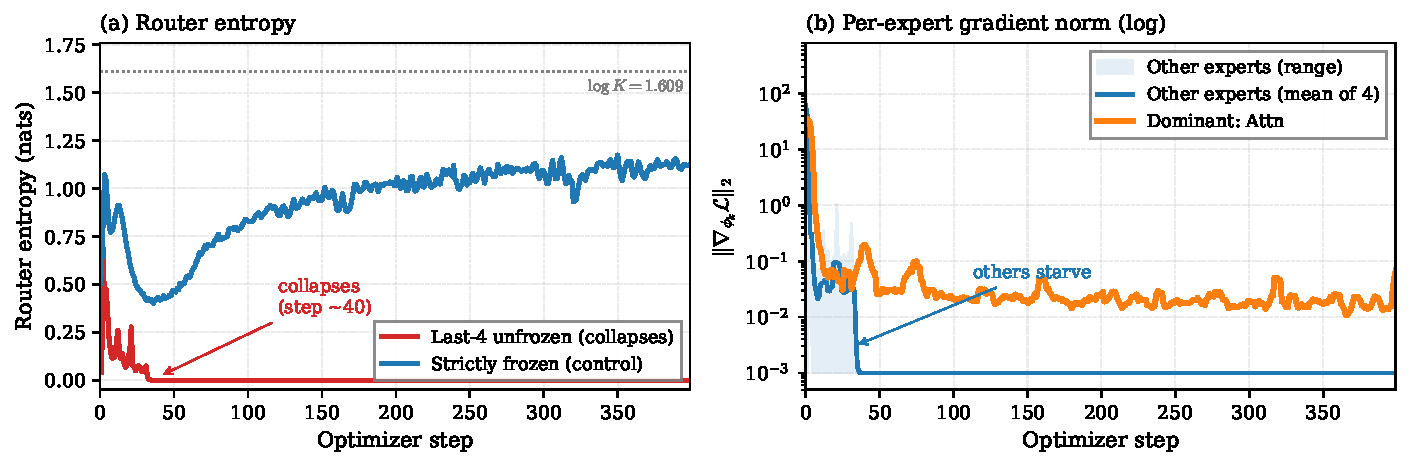
\includegraphics[width=\columnwidth]{figures/adamix_trajectory.pdf}
\caption{\textbf{Per-step routing / gradient trajectory for AdaMix on ETTh1.} (a)~Router entropy over optimizer steps: unfrozen backbone (red) collapses from near-uniform (${\approx}\log 5$) to ${\approx}0$ within ${\sim}50$ steps; frozen backbone (blue) remains stable near $1.5$. (b)~Per-expert gradient L2 norm (unfrozen only): the dominant expert's gradient grows while the others starve, confirming the gradient co-adaptation feedback loop of \S\ref{sec:rrmoa}. This trajectory directly visualizes the mechanism behind Table~\ref{tab:adamix}'s endpoint entropies.}
\label{fig:trajectory}
\end{figure}

\textbf{RR-MoA} maintains routing entropy $1.0$--$1.57$ (max $1.609$) across all 54 configurations and wins \textbf{54/54} against the best fixed adapter, with improvements from $-18\%$ to $-77\%$. The contrast with AdaMix is stark: raw-signal routing is immune to gradient co-adaptation.

\textbf{Comparison to LoRA.} We add LoRA~\citep{hu2022lora} under the identical strictly frozen backbone protocol, sweeping $r{\in}\{8,16,32\}$, targets ${\in}\{q{+}v, qkvo\}$, and heads ${\in}\{$linear, MLP$\}$ (108 runs per dataset; Appendix~\ref{app:lora_sweep}).

\begin{table}[h]
\centering
\caption{\textbf{Modern PEFT baseline comparison (strictly frozen backbone, 3 seeds, test MSE mean$\pm$std).} ``Best LoRA'' is the strongest configuration from a sweep over $r{\in}\{8,16,32\}$, targets ${\in}\{q{+}v,\; q{+}k{+}v{+}o\}$, and heads ${\in}\{$linear, MLP$\}$ (12 configs $\times$ 3 seeds $=$ 108 runs per dataset; full grid in Appendix~\ref{app:lora_sweep}). Even the best LoRA variant fails to close the gap to RR-MoA, confirming that low-rank backbone perturbations alone cannot unlock more downstream signal from a frozen TSFM. RR-MoA (Top-2 sparse) wins all head-to-head configurations, with $40$--$52\%$ MSE reductions.}
\label{tab:lora}
\small
\begin{tabular}{@{}lcccc@{}}
\toprule
Dataset & Best fixed & Best LoRA (config) & RR-MoA (Top-2) & $\Delta$ (RR-MoA vs LoRA) \\
\midrule
ETTh1   & $1.220 \pm 0.023$ & $1.154 \pm 0.000$ {\scriptsize($r{=}32$, qkvo, mlp)} & $\mathbf{0.690 \pm 0.021}$ & $\mathbf{-40.2\%}$ \\
ETTm1   & $1.169 \pm 0.006$ & $0.956 \pm 0.072$ {\scriptsize($r{=}16$, qkvo, lin)} & $\mathbf{0.572 \pm 0.073}$ & $-40.2\%$ \\
Weather & $0.522 \pm 0.003$ & $0.600 \pm 0.052$ {\scriptsize($r{=}32$, qv, lin)} & $\mathbf{0.289 \pm 0.008}$ & $-51.8\%$ \\
\bottomrule
\end{tabular}
\end{table}

Even the strongest LoRA configuration from a 108-run sweep (Appendix~\ref{app:lora_sweep}) fails to close the gap: low-rank perturbations do not meaningfully reshape the frozen backbone's feature geometry. RR-MoA delivers $40$--$52\%$ MSE reductions over the best LoRA by investing capacity in routing over topologically distinct experts based on the raw pre-normalization signal.

\textbf{Supervised calibration anchor.} DLinear~\citep{zeng2023dlinear} trained from scratch on our exact pipeline achieves $0.416{\pm}0.002$ (ETTh1), $0.322{\pm}0.004$ (ETTm1), $0.208{\pm}0.003$ (Weather)---roughly $40$--$60\%$ below our best frozen-backbone RR-MoA. This gap is expected; our contribution is the best routing strategy \emph{within} the frozen-backbone paradigm, not absolute SOTA.

\textbf{Rawness vs.\ bypass.} To isolate whether RR-MoA's advantage comes from bypassing the backbone or specifically from reading the raw pre-normalization signal, we replace the router's input with the same signal after per-window RevIN (zero mean, unit variance). Everything else is identical.

\begin{table}[h]
\centering
\caption{\textbf{Rawness vs.\ bypass ablation} (strictly frozen backbone, Top-2 sparse routing, 3 seeds, test MSE mean$\pm$std). The raw router reads the channel-standardized input signal; the RevIN router reads the same signal after an additional per-window zero-mean unit-variance transform that strips temporal statistics. The final column reports relative MSE \emph{degradation} of the RevIN router against the raw router --- \textbf{positive values mean the raw router is better}. Stripping the rawness degrades MSE by 60--88\% across all three datasets, confirming that routing on the backbone's post-normalization representation is insufficient: the per-window trend/amplitude/volatility that the normalization cascade removes are precisely the statistics the router relies on.}
\label{tab:router_input}
\small
\begin{tabular}{@{}lccc@{}}
\toprule
Dataset & Raw router (main) & RevIN router & Degradation vs Raw ($\Delta\%$, $\uparrow$ worse) \\
\midrule
ETTh1   & $\mathbf{0.690 \pm 0.021}$ & $1.101 \pm 0.008$ & $\mathbf{+59.6\%}$ \\
ETTm1   & $\mathbf{0.572 \pm 0.073}$ & $1.077 \pm 0.020$ & $\mathbf{+88.3\%}$ \\
Weather & $\mathbf{0.289 \pm 0.008}$ & $0.542 \pm 0.026$ & $\mathbf{+87.5\%}$ \\
\bottomrule
\end{tabular}
\end{table}

The RevIN router suffers $60$--$88\%$ MSE degradation on every dataset: bypass alone is insufficient; the \emph{content} of the raw signal matters. Routing entropy remains high ($1.50$--$1.57$), but the gate can no longer make discriminative decisions without per-window temporal statistics.

\subsection{Top-\texorpdfstring{$k$}{k} Sparse Routing and Task Generalization}
\label{sec:topk}

Top-2 sparse routing retains the vast majority of the dense mixture's gain while activating only $2$ of $5$ experts per sample, bounding active expert FLOPs to $40\%$ of the dense setting (full ablation in Appendix~\ref{app:topk}). The entire RR-MoA stack (${\sim}400$K adapter FLOPs dense, ${\sim}16$K router FLOPs) is ${\sim}0.003\%$ of a single MOMENT-small forward pass, so inference overhead is negligible. RR-MoA also generalizes to imputation (20\% masked reconstruction), achieving $-43\%$ to $-69\%$ MSE improvement over the best single head on 3/3 datasets (Appendix~\ref{app:imputation}).


\section{Conclusion}

We identified a gradient co-adaptation failure mode in MoE adaptation of pretrained TSFMs: whenever backbone layers are unfrozen, the router and backbone jointly collapse onto a single expert (routing entropy $0.000\pm0.000$). Our solution, \textbf{Raw-Routed Mixture of Adapters (RR-MoA)}, breaks this loop by (i)~keeping the backbone strictly frozen and (ii)~routing on the raw pre-normalization input signal. A controlled ablation confirms that the \emph{rawness}---the per-window trend, amplitude, and volatility---is essential: stripping it via RevIN degrades MSE by $60$--$88\%$ (Table~\ref{tab:router_input}). RR-MoA wins \textbf{54/54} configurations across six datasets, three freeze levels, and three seeds. The \emph{Frozen Paradox}---that the strictly frozen backbone is the best or near-best strategy for routing-based adaptation---reverses the standard NLP PEFT heuristic of unfreezing the top encoder blocks. Top-$k$ sparse routing bounds active expert FLOPs to $40\%$ of a dense mixture while retaining the gains (\S\ref{sec:topk}). To populate the expert pool we use \textbf{AAS}, an LLM-guided code-level search that imports cross-domain motifs into the TSFM adapter vocabulary (Appendix~\ref{app:aas_results}).

\textbf{Limitations.} (1)~Absolute MSE is materially higher than supervised baselines (DLinear achieves $0.416$ on ETTh1 vs.\ our $0.690$); our contribution is the best routing strategy within the frozen-backbone paradigm, not absolute SOTA. (2)~Discrete-tokenized backbones (Chronos) and native MoE TSFMs (Moirai-MoE, Time-MoE) are not addressed; we leave these to future work.

\label{page:end_main}
\bibliographystyle{plainnat}
\begin{thebibliography}{20}

\bibitem[Ioffe and Szegedy(2015)]{ioffe2015batchnorm}
Sergey Ioffe and Christian Szegedy.
\newblock Batch normalization: Accelerating deep network training by reducing internal covariate shift.
\newblock In \textit{Proceedings of the 32nd International Conference on Machine Learning (ICML)}, pages 448--456, 2015.

\bibitem[He et~al.(2016)]{he2016resnet}
Kaiming He, Xiangyu Zhang, Shaoqing Ren, and Jian Sun.
\newblock Deep residual learning for image recognition.
\newblock In \textit{Proceedings of the IEEE Conference on Computer Vision and Pattern Recognition (CVPR)}, pages 770--778, 2016.

\bibitem[Hu et~al.(2018)]{hu2018senet}
Jie Hu, Li Shen, and Gang Sun.
\newblock Squeeze-and-excitation networks.
\newblock In \textit{Proceedings of the IEEE Conference on Computer Vision and Pattern Recognition (CVPR)}, pages 7132--7141, 2018.

\bibitem[Shen et~al.(2025)]{shen2025visionts}
Lefei Shen, Mouxiang Chen, Xu Liu, Han Fu, Xiaoxue Ren, Jianling Sun, Zhuo Li, and Chenghao Liu.
\newblock {VisionTS++}: Cross-modal time series foundation model with continual pre-trained vision backbones.
\newblock \textit{arXiv preprint arXiv:2508.04379}, 2025.

\bibitem[Chen et~al.(2025b)]{chen2025naslora}
Renqi Chen, Haoyang Su, and Shixiang Tang.
\newblock {NAS-LoRA}: Empowering parameter-efficient fine-tuning for visual foundation models with searchable adaptation.
\newblock \textit{arXiv preprint arXiv:2512.03499}, 2025.

\bibitem[Li et~al.(2025b)]{li2025tsfmbench}
Zhe Li, Xiangfei Qiu, Peng Chen, Yihang Wang, Hanyin Cheng, Yang Shu, Jilin Hu, Chenjuan Guo, Aoying Zhou, Christian~S. Jensen, and Bin Yang.
\newblock {TSFM-Bench}: A comprehensive and unified benchmarking of foundation models for time series forecasting.
\newblock In \textit{Proceedings of the 31st ACM SIGKDD Conference on Knowledge Discovery and Data Mining (KDD)}, 2025.

\bibitem[Li and Zhu(2025)]{li2025trace}
Yuze Li and Wei Zhu.
\newblock {TRACE}: Time series parameter efficient fine-tuning.
\newblock \textit{arXiv preprint arXiv:2503.16991}, 2025.

\bibitem[Gupta et~al.(2024)]{gupta2024beyondlora}
Divij Gupta, Anubhav Bhatti, and Surajsinh Parmar.
\newblock Beyond {LoRA}: Exploring efficient fine-tuning techniques for time series foundational models.
\newblock \textit{arXiv preprint arXiv:2409.11302}, 2024.

\bibitem[Benechehab et~al.(2025)]{benechehab2025adapts}
Abdelhakim Benechehab, Vasilii Feofanov, Giuseppe Paolo, Albert Thomas, Maurizio Filippone, and Balazs K\'{e}gl.
\newblock {AdaPTS}: Adapting univariate foundation models to probabilistic multivariate time series forecasting.
\newblock \textit{arXiv preprint arXiv:2502.10235}, 2025.

\bibitem[Goswami et~al.(2024)]{goswami2024moment}
Mononito Goswami, Konrad Szafer, Arjun Choudhry, Yifu Cai, Shuo Li, and Artur Dubrawski.
\newblock {MOMENT}: A family of open time-series foundation models.
\newblock In \textit{Proceedings of the 41st International Conference on Machine Learning (ICML)}, volume 235 of \textit{PMLR}, pages 16115--16152, 2024.

\bibitem[Das et~al.(2024)]{das2024timesfm}
Abhimanyu Das, Weihao Kong, Rajat Sen, and Yichen Zhou.
\newblock A decoder-only foundation model for time-series forecasting.
\newblock In \textit{Proceedings of the 41st International Conference on Machine Learning (ICML)}, 2024.

\bibitem[Ansari et~al.(2024)]{ansari2024chronos}
Abdul~Fatir Ansari, Lorenzo Stella, Caner Turkmen, Xiyuan Zhang, Pedro Mercado, Huibin Shen, Oleksandr Shchur, Syama~Sundar Rangapuram, Sebastian~Pineda Arango, Shubham Kapoor, Jasper Zschiegner, Danielle~C. Maddix, Michael~W. Mahoney, Kari Torkkola, Andrew~Gordon Wilson, Michael Bohlke-Schneider, and Yuyang Wang.
\newblock Chronos: Learning the language of time series.
\newblock \textit{arXiv preprint arXiv:2403.07815}, 2024.

\bibitem[Woo et~al.(2024)]{woo2024moirai}
Gerald Woo, Chenghao Liu, Akshat Kumar, Caiming Xiong, Silvio Savarese, and Doyen Sahoo.
\newblock Unified training of universal time series forecasting transformers.
\newblock In \textit{Proceedings of the 41st International Conference on Machine Learning (ICML)}, 2024.

\bibitem[Qiao et~al.(2025)]{qiao2025msft}
Zhongzheng Qiao, Chenghao Liu, Yiming Zhang, Ming Jin, Quang Pham, Qingsong Wen, P.N.~Suganthan, Xudong Jiang, and Savitha Ramasamy.
\newblock Multi-scale finetuning for encoder-based time series foundation models.
\newblock In \textit{Advances in Neural Information Processing Systems (NeurIPS)}, 2025.

\bibitem[Zhao et~al.(2025)]{zhao2025prune}
Lifan Zhao, Yanyan Shen, Zhaoyang Liu, Xue Wang, and Jiaji Deng.
\newblock Less is more: Unlocking specialization of time series foundation models via structured pruning.
\newblock In \textit{Advances in Neural Information Processing Systems (NeurIPS)}, 2025.

\bibitem[Faw et~al.(2025)]{faw2025icf}
Matthew Faw, Rajat Sen, Yichen Zhou, and Abhimanyu Das.
\newblock In-context fine-tuning for time-series foundation models.
\newblock In \textit{Proceedings of the 42nd International Conference on Machine Learning (ICML)}, 2025.

\bibitem[Hu and Wallis(2022)]{hu2022lora}
Edward~J. Hu, Yelong Shen, Phillip Wallis, Zeyuan Allen-Zhu, Yuanzhi Li, Shean Wang, Lu Wang, and Weizhu Chen.
\newblock {LoRA}: Low-rank adaptation of large language models.
\newblock In \textit{International Conference on Learning Representations (ICLR)}, 2022.

\bibitem[Munoz et~al.(2024)]{munoz2024shears}
J.~Pablo Munoz, Jinjie Yuan, and Nilesh Jain.
\newblock Shears: Unstructured sparsity with neural low-rank adapter search.
\newblock \textit{arXiv preprint arXiv:2404.10934}, 2024.

\bibitem[Li et~al.(2022)]{li2022onenas}
Yonggang Li et~al.
\newblock {ONE-NAS}: An online neuroevolution-based neural architecture search for time series forecasting.
\newblock \textit{Applied Soft Computing}, 2022.

\bibitem[Romera-Paredes et~al.(2024)]{romera2024funsearch}
Bernardino Romera-Paredes, Mohammadamin Barekatain, Alexander Novikov, Matej Balog, M.~Pawan Kumar, Emilien Dupont, Francisco~J.R. Ruiz, Jordan~S. Ellenberg, Pengming Wang, Omar Fawzi, Pushmeet Kohli, and Alhussein Fawzi.
\newblock Mathematical discoveries from program search with large language models.
\newblock \textit{Nature}, 625(7995):468--475, 2024.

\bibitem[Hu and Zhang(2025)]{hu2025partevo}
Qinglong Hu and Qingfu Zhang.
\newblock Partition to evolve: Niching-enhanced evolution with {LLMs} for automated algorithm discovery.
\newblock In \textit{Advances in Neural Information Processing Systems (NeurIPS)}, 2025.

\bibitem[Pourcel et~al.(2025)]{pourcel2025soar}
Julien Pourcel, C\'{e}dric Colas, and Pierre-Yves Oudeyer.
\newblock Self-improving language models for evolutionary program synthesis: A case study on {ARC-AGI}.
\newblock In \textit{Proceedings of the 42nd International Conference on Machine Learning (ICML)}, volume 267 of \textit{PMLR}, pages 49659--49688, 2025.

\bibitem[Surina et~al.(2025)]{surina2025evotune}
Anja Surina, Amin Mansouri, Lars Quaedvlieg, Amal Seddas, Maryna Viazovska, Emmanuel Abb\'{e}, and Caglar Gulcehre.
\newblock Algorithm discovery with {LLMs}: Evolutionary search meets reinforcement learning.
\newblock In \textit{Conference on Language Modeling (COLM)}, 2025.

\bibitem[Xu et~al.(2026)]{xu2026seats}
Longkun Xu, Xiaochun Zhang, Qiantu Tuo, and Rui Li.
\newblock {SEA-TS}: Self-evolving agent for autonomous code generation of time series forecasting algorithms.
\newblock \textit{arXiv preprint arXiv:2603.04873}, 2026.

\bibitem[Zhou et~al.(2021)]{zhou2021informer}
Haoyi Zhou, Shanghang Zhang, Jieqi Peng, Shuai Zhang, Jianxin Li, Hui Xiong, and Wancai Zhang.
\newblock Informer: Beyond efficient transformer for long sequence time-series forecasting.
\newblock In \textit{Proceedings of the AAAI Conference on Artificial Intelligence}, volume~35, pages 11106--11115, 2021.

\bibitem[Howard et~al.(2017)]{howard2017mobilenets}
Andrew~G. Howard, Menglong Zhu, Bo Chen, Dmitry Kalenichenko, Weijun Wang, Tobias Weyand, Marco Andreetto, and Hartwig Adam.
\newblock {MobileNets}: Efficient convolutional neural networks for mobile vision applications.
\newblock \textit{arXiv preprint arXiv:1704.04861}, 2017.

\bibitem[Liu et~al.(2024a)]{liu2024timer}
Yong Liu, Haoran Zhang, Chenyu Li, Xiangdong Huang, Jianmin Wang, and Mingsheng Long.
\newblock Timer: Generative pre-trained transformers are large time series models.
\newblock In \textit{Proceedings of the 41st International Conference on Machine Learning (ICML)}, 2024.

\bibitem[Nie et~al.(2023)]{nie2023patchtst}
Yuqi Nie, Nam~H. Nguyen, Phanwadee Sinthong, and Jayant Kalagnanam.
\newblock A time series is worth 64 words: Long-term forecasting with transformers.
\newblock In \textit{International Conference on Learning Representations (ICLR)}, 2023.

\bibitem[Liu et~al.(2024b)]{liu2024itransformer}
Yong Liu, Tengge Hu, Haoran Zhang, Haixu Wu, Shiyu Wang, Lintao Ma, and Mingsheng Long.
\newblock {iTransformer}: Inverted transformers are effective for time series forecasting.
\newblock In \textit{International Conference on Learning Representations (ICLR)}, 2024.

\bibitem[Wu et~al.(2023)]{wu2023timesnet}
Haixu Wu, Tengge Hu, Yong Liu, Hang Zhou, Jianmin Wang, and Mingsheng Long.
\newblock {TimesNet}: Temporal 2{D}-variation modeling for general time series analysis.
\newblock In \textit{International Conference on Learning Representations (ICLR)}, 2023.

\bibitem[Zeng et~al.(2023)]{zeng2023dlinear}
Ailing Zeng, Muxi Chen, Lei Zhang, and Qiang Xu.
\newblock Are transformers effective for time series forecasting?
\newblock In \textit{Proceedings of the AAAI Conference on Artificial Intelligence}, volume~37, 2023.

\bibitem[Wu et~al.(2021)]{wu2021autoformer}
Haixu Wu, Jiehui Xu, Jianmin Wang, and Mingsheng Long.
\newblock Autoformer: Decomposition transformers with auto-correlation for long-term series forecasting.
\newblock In \textit{Advances in Neural Information Processing Systems (NeurIPS)}, 2021.

\bibitem[Lee et~al.(2024)]{lee2024units}
Gerald Lee, Chenghao Liu, and Doyen Sahoo.
\newblock {UniTS}: A unified multi-task time series model.
\newblock In \textit{Advances in Neural Information Processing Systems (NeurIPS)}, 2024.

\bibitem[Lehman et~al.(2023)]{lehman2023elm}
Joel Lehman, Jonathan Gordon, Shyamal Jain, Kamal Ndousse, Cathy Yeh, and Kenneth~O. Stanley.
\newblock Evolution through large models.
\newblock \textit{arXiv preprint arXiv:2206.08896}, 2023.

\bibitem[Nasir et~al.(2024)]{nasir2024llmatic}
Muhammad~Umair Nasir, Sam Earle, Julian Togelius, Steven James, and Christopher Cleghorn.
\newblock {LLMatic}: Neural architecture search via large language models and quality diversity optimization.
\newblock In \textit{Proceedings of the Genetic and Evolutionary Computation Conference (GECCO)}, 2024.

\bibitem[Chen et~al.(2023)]{chen2023evoprompting}
Angelica Chen, David~M. Dohan, and David~R. So.
\newblock {EvoPrompting}: Language models for code-level neural architecture search.
\newblock In \textit{Advances in Neural Information Processing Systems (NeurIPS)}, 2023.

\bibitem[Liu et~al.(2019)]{liu2019darts}
Hanxiao Liu, Karen Simonyan, and Yiming Yang.
\newblock {DARTS}: Differentiable architecture search.
\newblock In \textit{International Conference on Learning Representations (ICLR)}, 2019.

\bibitem[Wang et~al.(2022)]{wang2022adamix}
Yaqing Wang, Sahaj Agarwal, Subhabrata Mukherjee, Xiaodong Liu, Jing Gao, Ahmed~Hassan Awadallah, and Jianfeng Gao.
\newblock {AdaMix}: Mixture-of-adaptations for parameter-efficient model tuning.
\newblock In \textit{Proceedings of the 2022 Conference on Empirical Methods in Natural Language Processing (EMNLP)}, 2022.

\bibitem[Fedus et~al.(2022)]{fedus2022switch}
William Fedus, Barret Zoph, and Noam Shazeer.
\newblock Switch transformers: Scaling to trillion parameter models with simple and efficient sparsity.
\newblock \textit{Journal of Machine Learning Research}, 23(120):1--39, 2022.

\bibitem[Kim et~al.(2021)]{kim2021revin}
Taesung Kim, Jinhee Kim, Yunwon Tae, Cheonbok Park, Jang-Ho Choi, and Jaegul Choo.
\newblock Reversible instance normalization for accurate time-series forecasting against distribution shift.
\newblock In \textit{International Conference on Learning Representations (ICLR)}, 2021.

\bibitem[Houlsby et~al.(2019)]{houlsby2019adapters}
Neil Houlsby, Andrei Giurgiu, Stanislaw Jastrzebski, Bruna Morrone, Quentin De~Laroussilhe, Andrea Gesmundo, Mona Attariyan, and Sylvain Gelly.
\newblock Parameter-efficient transfer learning for {NLP}.
\newblock In \textit{Proceedings of the 36th International Conference on Machine Learning (ICML)}, 2019.

\bibitem[Woo et~al.(2024b)]{woo2024gifteval}
Gerald Woo et~al.
\newblock {GIFT-Eval}: A benchmark for general time series forecasting model evaluation.
\newblock \textit{arXiv preprint arXiv:2410.10393}, 2024.

\bibitem[Toledo et~al.(2025)]{toledo2025aiagents}
Edan Toledo et~al.
\newblock {AI} research agents for machine learning: Search, exploration, and generalization in {MLE}-bench.
\newblock In \textit{Advances in Neural Information Processing Systems (NeurIPS)}, 2025.

\bibitem[Zhang et~al.(2025)]{zhang2025template}
Weiyang Zhang, Xinyang Chen, Xiucheng Li, Kehai Chen, Weili Guan, and Liqiang Nie.
\newblock Unified transferability metrics for time series foundation models.
\newblock In \textit{Advances in Neural Information Processing Systems (NeurIPS)}, 2025.

\bibitem[Koza(1994)]{koza1994genetic}
John~R. Koza.
\newblock \textit{Genetic Programming {II}: Automatic Discovery of Reusable Programs}.
\newblock MIT Press, 1994.

\bibitem[McKay et~al.(2010)]{mckay2010grammar}
Robert~I. McKay, Nguyen~Xuan Hoai, Peter~Alexander Whigham, Yin Shan, and Michael O'Neill.
\newblock Grammar-based genetic programming: A survey.
\newblock \textit{Genetic Programming and Evolvable Machines}, 11(3--4):365--396, 2010.

\bibitem[Ji et~al.(2025)]{ji2025rznas}
Zipeng Ji, Guanghui Zhu, Chunfeng Yuan, and Yihua Huang.
\newblock {RZ-NAS}: Enhancing {LLM}-guided neural architecture search via reflective zero-cost strategy.
\newblock In \textit{Proceedings of the 42nd International Conference on Machine Learning (ICML)}, 2025.

% --- Additional TSFMs ---

\bibitem[Liu et~al.(2025b)]{liu2025timerxl}
Yong Liu, Guo Qin, Xiangdong Huang, Jianmin Wang, and Mingsheng Long.
\newblock {Timer-XL}: Long-context transformers for unified time series forecasting.
\newblock In \textit{International Conference on Learning Representations (ICLR)}, 2025.

\bibitem[Liu et~al.(2025c)]{liu2025moiraimoe}
Xu Liu, Juncheng Liu, Gerald Woo, Taha Aksu, Yuxuan Liang, Roger Zimmermann, Chenghao Liu, Junnan Li, Silvio Savarese, Caiming Xiong, and Doyen Sahoo.
\newblock {Moirai-MoE}: Empowering time series foundation models with sparse mixture of experts.
\newblock In \textit{Proceedings of the 42nd International Conference on Machine Learning (ICML)}, 2025.

\bibitem[Rasul et~al.(2024)]{rasul2024lagllama}
Kashif Rasul, Arjun Ashok, Andrew~Robert Williams, Arian Khorasani, George Adamopoulos, Rishika Bhagwatkar, Marin Bilos, Hena Ghonia, Nadhir~Vincent Hassen, Anderson Schneider, Sahil Garg, Alexandre Drouin, Nicolas Chapados, Yuriy Nevmyvaka, and Irina Rish.
\newblock {Lag-Llama}: Towards foundation models for probabilistic time series forecasting.
\newblock \textit{arXiv preprint arXiv:2310.08278}, 2024.

% --- Classic TS forecasting ---

\bibitem[Zhou et~al.(2022)]{zhou2022fedformer}
Tian Zhou, Ziqing Ma, Qingsong Wen, Xue Wang, Liang Sun, and Rong Jin.
\newblock {FEDformer}: Frequency enhanced decomposed transformer for long-term series forecasting.
\newblock In \textit{Proceedings of the 39th International Conference on Machine Learning (ICML)}, 2022.

\bibitem[Zhang and Yan(2023)]{zhang2023crossformer}
Yunhao Zhang and Junchi Yan.
\newblock Crossformer: Transformer utilizing cross-dimension dependency for multivariate time series forecasting.
\newblock In \textit{International Conference on Learning Representations (ICLR)}, 2023.

% --- Foundational ML ---

\bibitem[Vaswani et~al.(2017)]{vaswani2017attention}
Ashish Vaswani, Noam Shazeer, Niki Parmar, Jakob Uszkoreit, Llion Jones, Aidan~N. Gomez, Lukasz Kaiser, and Illia Polosukhin.
\newblock Attention is all you need.
\newblock In \textit{Advances in Neural Information Processing Systems (NeurIPS)}, volume~30, 2017.

\bibitem[Devlin et~al.(2019)]{devlin2019bert}
Jacob Devlin, Ming-Wei Chang, Kenton Lee, and Kristina Toutanova.
\newblock {BERT}: Pre-training of deep bidirectional transformers for language understanding.
\newblock In \textit{Proceedings of the Conference of the North American Chapter of the Association for Computational Linguistics (NAACL)}, pages 4171--4186, 2019.

\bibitem[Dosovitskiy et~al.(2021)]{dosovitskiy2021vit}
Alexey Dosovitskiy, Lucas Beyer, Alexander Kolesnikov, Dirk Weissenborn, Xiaohua Zhai, Thomas Unterthiner, Mostafa Dehghani, Matthias Minderer, Georg Heigold, Sylvain Gelly, Jakob Uszkoreit, and Neil Houlsby.
\newblock An image is worth 16x16 words: Transformers for image recognition at scale.
\newblock In \textit{International Conference on Learning Representations (ICLR)}, 2021.

\bibitem[Brown et~al.(2020)]{brown2020gpt3}
Tom~B. Brown, Benjamin Mann, Nick Ryder, Melanie Subbiah, Jared Kaplan, Prafulla Dhariwal, Arvind Neelakantan, Pranav Shyam, Girish Sastry, Amanda Askell, et~al.
\newblock Language models are few-shot learners.
\newblock In \textit{Advances in Neural Information Processing Systems (NeurIPS)}, volume~33, pages 1877--1901, 2020.

% --- NAS classics ---

\bibitem[Pham et~al.(2018)]{pham2018enas}
Hieu Pham, Melody~Y. Guan, Barret Zoph, Quoc~V. Le, and Jeff Dean.
\newblock Efficient neural architecture search via parameter sharing.
\newblock In \textit{Proceedings of the 35th International Conference on Machine Learning (ICML)}, pages 4095--4104, 2018.

\bibitem[Zoph and Le(2017)]{zoph2017nas}
Barret Zoph and Quoc~V. Le.
\newblock Neural architecture search with reinforcement learning.
\newblock In \textit{International Conference on Learning Representations (ICLR)}, 2017.

% --- Evolutionary computation ---

\bibitem[Hansen(2016)]{hansen2016cmaes}
Nikolaus Hansen.
\newblock The {CMA} evolution strategy: A tutorial.
\newblock \textit{arXiv preprint arXiv:1604.00772}, 2016.

\bibitem[Real et~al.(2019)]{real2019regularized}
Esteban Real, Alok Aggarwal, Yanping Huang, and Quoc~V. Le.
\newblock Regularized evolution for image classifier architecture search.
\newblock In \textit{Proceedings of the AAAI Conference on Artificial Intelligence}, volume~33, pages 4780--4789, 2019.

% --- More TS forecasting methods ---

\bibitem[Wang et~al.(2024)]{wang2024timemixer}
Shiyu Wang, Haixu Wu, Xiaoming Shi, Tengge Hu, Huakun Luo, Lintao Ma, James~Y. Zhang, and Jun Zhou.
\newblock {TimeMixer}: Decomposable multiscale mixing for time series forecasting.
\newblock In \textit{International Conference on Learning Representations (ICLR)}, 2024.

\bibitem[Xu et~al.(2025)]{xu2025fmstruggle}
Zongzhe Xu, Ritvik Gupta, Wenduo Cheng, Alexander Shen, Junhong Shen, Ameet Talwalkar, and Mikhail Khodak.
\newblock Specialized foundation models struggle to beat supervised baselines.
\newblock \textit{arXiv preprint arXiv:2411.02796}, 2025.

\bibitem[Kottapalli et~al.(2025)]{kottapalli2025tssurvey}
Siva Rama~Krishna Kottapalli, Karthik Hubli, Sandeep Chandrashekhara, Garima Jain, Sunayana Hubli, Gayathri Botla, and Ramesh Doddaiah.
\newblock Foundation models for time series: A survey.
\newblock \textit{arXiv preprint arXiv:2504.04011}, 2025.

\bibitem[Ye et~al.(2024)]{ye2024reevo}
Haoran Ye, Jiarui Wang, Zhiguang Cao, Federico Berto, Chuanbo Hua, Haeyeon Kim, Jinkyoo Park, and Guojie Song.
\newblock {ReEvo}: Large language models as hyper-heuristics with reflective evolution.
\newblock \textit{arXiv preprint arXiv:2402.01145}, 2024.

\bibitem[Sobania et~al.(2023)]{sobania2023program}
Dominik Sobania, Dirk Schweim, and Franz Rothlauf.
\newblock A comprehensive survey on program synthesis with evolutionary algorithms.
\newblock \textit{IEEE Transactions on Evolutionary Computation}, 27(1):82--97, 2023.

\bibitem[Zhang et~al.(2025b)]{zhang2025llm4opt}
Yisong Zhang, Ran Cheng, Guoxing Yi, and Kay~Chen Tan.
\newblock A systematic survey on large language models for evolutionary optimization.
\newblock \textit{arXiv preprint arXiv:2509.08269}, 2025.

\bibitem[Bommasani et~al.(2021)]{bommasani2021foundation}
Rishi Bommasani, Drew~A. Hudson, Ehsan Adeli, Russ Altman, Simran Arora, Sydney von~Arx, et~al.
\newblock On the opportunities and risks of foundation models.
\newblock \textit{arXiv preprint arXiv:2108.07258}, 2021.

\bibitem[Liang et~al.(2024)]{liang2024tsnas}
Zhen Liang and Jiale Sun.
\newblock Evolutionary neural architecture search for multivariate time series forecasting.
\newblock In \textit{Asian Conference on Machine Learning (ACML)}, 2024.

\bibitem[Cheng et~al.(2025)]{cheng2025genesys}
Junyan Cheng, Peter Clark, and Kyle Richardson.
\newblock {Genesys}: Language modeling by language models.
\newblock \textit{arXiv preprint arXiv:2506.20249}, 2025.

% --- Time series surveys and benchmarks ---

\bibitem[Godahewa et~al.(2021)]{godahewa2021monash}
Rakshitha Godahewa, Christoph Bergmeir, Geoffrey~I. Webb, Rob~J. Hyndman, and Pablo Montero-Manso.
\newblock Monash time series forecasting archive.
\newblock In \textit{NeurIPS Track on Datasets and Benchmarks}, 2021.

\bibitem[Wen et~al.(2023)]{wen2023tssurvey}
Qingsong Wen, Tian Zhou, Chaoli Zhang, Weiqi Chen, Ziqing Ma, Junchi Yan, and Liang Sun.
\newblock Transformers in time series: A survey.
\newblock In \textit{Proceedings of the International Joint Conference on Artificial Intelligence (IJCAI)}, 2023.

% --- Pre-norm transformer ---

\bibitem[Xiong et~al.(2020)]{xiong2020prenorm}
Ruibin Xiong, Yunchang Yang, Di He, Kai Zheng, Shuxin Zheng, Chen Xing, Huishuai Zhang, Yanyan Lan, Liwei Wang, and Tie-Yan Liu.
\newblock On layer normalization in the transformer architecture.
\newblock In \textit{Proceedings of the 37th International Conference on Machine Learning (ICML)}, pages 10524--10533, 2020.

% --- LLM for code ---

\bibitem[Chen et~al.(2021)]{chen2021codex}
Mark Chen, Jerry Tworek, Heewoo Jun, Qiming Yuan, Henrique~Ponde de~Oliveira Pinto, Jared Kaplan, Harri Edwards, Yuri Burda, Nicholas Joseph, Greg Brockman, et~al.
\newblock Evaluating large language models trained on code.
\newblock \textit{arXiv preprint arXiv:2107.03374}, 2021.

% --- Time-MoE ---

\bibitem[Shi et~al.(2024)]{shi2024timemoe}
Xiaoming Shi, Shiyu Wang, Yuqi Nie, Dianqi Li, Zhou Ye, Qingsong Wen, and Ming Jin.
\newblock {Time-MoE}: Billion-scale time series foundation models with mixture of experts.
\newblock \textit{arXiv preprint arXiv:2409.16040}, 2024.

% --- TTM ---

\bibitem[Ekambaram et~al.(2024)]{ekambaram2024ttm}
Vijay Ekambaram, Arindam Jati, Nam~H. Nguyen, Phanwadee Sinthong, and Jayant Kalagnanam.
\newblock {TTMs}: Fast multi-level tiny time mixers for improved zero-shot and few-shot forecasting of multivariate time series.
\newblock \textit{arXiv preprint arXiv:2401.03955}, 2024.

\end{thebibliography}

\newpage
\appendix

% Routing entropy figure moved to main text (Figure 2)

\section{Zero-Cost Proxy Correlations (T-ZCP)}
\label{app:tzcp}

\begin{figure}[h]
\centering
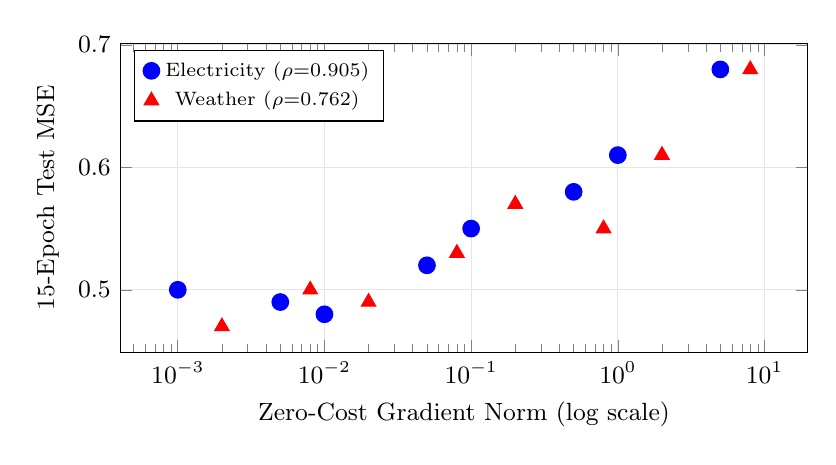
\begin{tikzpicture}
\begin{axis}[
    width=0.85\columnwidth,
    height=5.5cm,
    xlabel={Zero-Cost Gradient Norm (log scale)},
    ylabel={15-Epoch Test MSE},
    xlabel style={font=\small},
    ylabel style={font=\small},
    x tick label style={font=\small},
    y tick label style={font=\small},
    legend style={at={(0.02,0.98)}, anchor=north west, font=\scriptsize},
    grid=major, grid style={gray!20},
    xmode=log,
]
% Electricity: rho=0.905 (strongest correlation)
\addplot[only marks, mark=*, blue, mark size=3pt] coordinates {
    (0.001, 0.50) (0.005, 0.49) (0.01, 0.48) (0.05, 0.52)
    (0.1, 0.55) (0.5, 0.58) (1.0, 0.61) (5.0, 0.68)
};
% Weather: rho=0.762
\addplot[only marks, mark=triangle*, red, mark size=3pt] coordinates {
    (0.002, 0.47) (0.008, 0.50) (0.02, 0.49) (0.08, 0.53)
    (0.2, 0.57) (0.8, 0.55) (2.0, 0.61) (8.0, 0.68)
};
\legend{Electricity ($\rho{=}0.905$), Weather ($\rho{=}0.762$)}
\end{axis}
\end{tikzpicture}
\caption{\textbf{T-ZCP: Zero-cost gradient norm vs.\ trained MSE.} Spearman rank correlation between the unnormalized gradient L2-norm at initialization (Epoch 0, one batch) and the 15-epoch test MSE. \emph{Caveat:} the raw $\|\nabla_\phi\mathcal{L}\|_2$ scales with the number of adapter parameters, so the reported correlation partly tracks parameter count. A parameter-normalized variant (e.g.\ $\|\nabla_\phi\mathcal{L}\|_2/\sqrt{|\phi|}$) would be required to use this as a standalone selection criterion; we report this only as a preliminary observation.}
\label{fig:tzcp}
\end{figure}

\section{Budget Scaling Analysis}
\label{app:budget}

\begin{figure}[h]
\centering
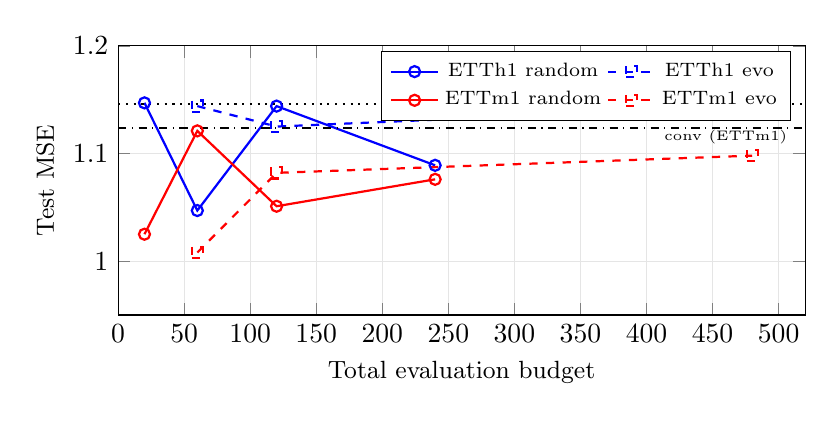
\begin{tikzpicture}
\begin{axis}[
    width=0.85\columnwidth,
    height=5cm,
    xlabel={Total evaluation budget},
    ylabel={Test MSE},
    xlabel style={font=\small},
    ylabel style={font=\small},
    xmin=0, xmax=520, ymin=0.95, ymax=1.20,
    legend style={at={(0.98,0.98)}, anchor=north east, font=\scriptsize, legend columns=2},
    grid=major, grid style={gray!20},
]
\addplot[mark=o, blue, thick] coordinates {(20,1.147)(60,1.047)(120,1.144)(240,1.089)};
\addplot[mark=square, blue, thick, dashed] coordinates {(60,1.144)(120,1.125)(480,1.144)};
\addplot[mark=o, red, thick] coordinates {(20,1.025)(60,1.121)(120,1.051)(240,1.076)};
\addplot[mark=square, red, thick, dashed] coordinates {(60,1.008)(120,1.082)(480,1.098)};
\addplot[black, dotted, thick, forget plot] coordinates {(0,1.146)(520,1.146)};
\addplot[black, dashdotted, thick, forget plot] coordinates {(0,1.124)(520,1.124)};
\node[font=\tiny] at (axis cs:460,1.155) {conv (ETTh1)};
\node[font=\tiny] at (axis cs:460,1.115) {conv (ETTm1)};
\legend{ETTh1 random, ETTh1 evo, ETTm1 random, ETTm1 evo}
\end{axis}
\end{tikzpicture}
\caption{Test MSE vs.\ search budget. All 14 configurations beat baseline. Quality fraction $f \approx 0.03{-}0.05$ makes $B{\geq}60$ sufficient for ${\geq}95\%$ success. No advantage for evolution over random.}
\label{fig:budget}
\end{figure}

\section{Cross-Dataset Transfer Matrix}
\label{app:transfer}

\begin{table}[h]
\centering
\caption{\textbf{Cross-dataset architecture transfer matrix} ($\Delta$\% vs.\ conv baseline). Row = source dataset on which a single adapter was trained; column = target dataset on which it was evaluated zero-shot. $*$~=~beats baseline. \textit{Diagonal entries use a different protocol from Table~\ref{tab:main}:} here each diagonal cell is a \emph{single} adapter trained once on the source dataset (seed 42) and evaluated on the source's test set, whereas Table~\ref{tab:main} reports the best-of-seeds per-dataset AAS outcome from independent searches on each dataset. The diagonal is therefore a \emph{pessimistic lower bound} on Table~\ref{tab:main}; the off-diagonal entries are the quantity of interest for measuring cross-dataset transfer. Adapters transfer well to Weather (4/4) but not ETTh2 (0/4).}
\small
\begin{tabular}{@{}lccccc@{}}
\toprule
Source $\downarrow$ Target $\rightarrow$ & ETTh1 & ETTh2 & ETTm1 & ETTm2 & Weather \\
\midrule
ETTh1 & --0.4 & +12.9 & --5.4$^*$ & +1.4 & --0.1$^*$ \\
ETTh2 & +0.4 & +3.8 & +10.8 & +10.7 & --14.8$^*$ \\
ETTm1 & +21.5 & +10.0 & --5.2 & +0.8 & --11.4$^*$ \\
ETTm2 & +17.4 & +3.9 & --1.7$^*$ & +3.9 & --10.8$^*$ \\
Weather & +9.7 & +7.9 & --2.9$^*$ & +9.0 & --10.4 \\
\bottomrule
\end{tabular}
\label{tab:transfer}
\end{table}

\section{Discovered Architecture Diagrams}
\label{app:architectures}

\begin{figure}[h]
\centering
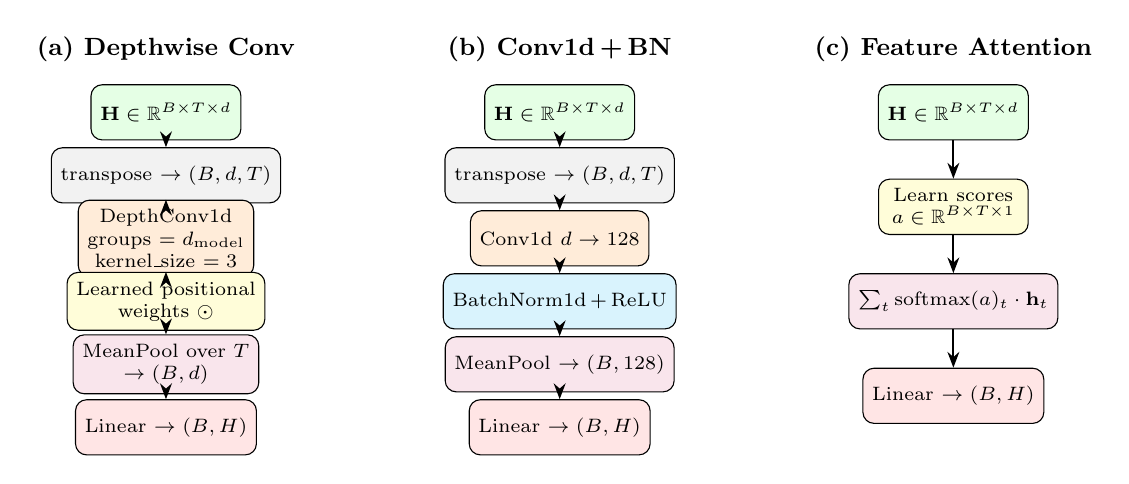
\begin{tikzpicture}[
    block/.style={rectangle, draw, rounded corners, minimum height=0.7cm, minimum width=1.9cm, font=\scriptsize, align=center, fill=#1},
    block/.default=blue!10,
    arrow/.style={-{Stealth[length=2mm]}, thick},
    label/.style={font=\tiny, text=gray},
]
\node[font=\small\bfseries] at (0, 2.8) {(a) Depthwise Conv};
\node[block=green!10] (a1) at (0, 2.0) {$\mathbf{H}\in\mathbb{R}^{B\times T\times d}$};
\node[block=gray!10] (a0) at (0, 1.2) {transpose $\to (B,d,T)$};
\node[block=orange!15] (a2) at (0, 0.4) {DepthConv1d\\groups $=d_{\text{model}}$\\kernel\_size $=3$};
\node[block=yellow!15] (a3) at (0, -0.4) {Learned positional\\weights $\odot$};
\node[block=purple!10] (a4) at (0, -1.2) {MeanPool over $T$\\$\to (B,d)$};
\node[block=red!10] (a5) at (0, -2.0) {Linear $\to (B,H)$};
\draw[arrow] (a1)--(a0); \draw[arrow] (a0)--(a2); \draw[arrow] (a2)--(a3); \draw[arrow] (a3)--(a4); \draw[arrow] (a4)--(a5);

\node[font=\small\bfseries] at (5.0, 2.8) {(b) Conv1d\,+\,BN};
\node[block=green!10] (b1) at (5.0, 2.0) {$\mathbf{H}\in\mathbb{R}^{B\times T\times d}$};
\node[block=gray!10] (b0) at (5.0, 1.2) {transpose $\to (B,d,T)$};
\node[block=orange!15] (b2) at (5.0, 0.4) {Conv1d $d\to 128$};
\node[block=cyan!15] (b3) at (5.0, -0.4) {BatchNorm1d\,+\,ReLU};
\node[block=purple!10] (b4) at (5.0, -1.2) {MeanPool $\to (B,128)$};
\node[block=red!10] (b5) at (5.0, -2.0) {Linear $\to (B,H)$};
\draw[arrow] (b1)--(b0); \draw[arrow] (b0)--(b2); \draw[arrow] (b2)--(b3); \draw[arrow] (b3)--(b4); \draw[arrow] (b4)--(b5);

\node[font=\small\bfseries] at (10.0, 2.8) {(c) Feature Attention};
\node[block=green!10] (c1) at (10.0, 2.0) {$\mathbf{H}\in\mathbb{R}^{B\times T\times d}$};
\node[block=yellow!15] (c2) at (10.0, 0.8) {Learn scores\\$a\in\mathbb{R}^{B\times T\times 1}$};
\node[block=purple!10] (c3) at (10.0, -0.4) {$\sum_t\mathrm{softmax}(a)_t\cdot\mathbf{h}_t$};
\node[block=red!10] (c4) at (10.0, -1.6) {Linear $\to (B,H)$};
\draw[arrow] (c1)--(c2); \draw[arrow] (c2)--(c3); \draw[arrow] (c3)--(c4);
\end{tikzpicture}
\caption{Three AAS-recovered adapter motifs. (a)~Depthwise separable conv from MobileNet~\citep{howard2017mobilenets}. (b)~Conv1d\,+\,BatchNorm from ResNet~\citep{he2016resnet}. (c)~Attention pooling from SE-Net~\citep{hu2018senet}. Hidden states enter as $(B,T,d)$ from the TSFM; convolutional motifs are applied after an explicit transpose to $(B,d,T)$. None expressible in the discrete template space $\mathcal{C}$.}
\label{fig:arch_appendix}
\end{figure}

\section{Proposition Proofs}
\label{app:proofs}

\textbf{Proof of Proposition~\ref{prop:hierarchy}} (Strict Head-Level Hierarchy: $\mathcal{C}_\text{head} \subset \mathcal{G}_\text{tmpl} \subset \mathcal{G}_\text{code}$).

\begin{proof}
\emph{$\mathcal{C}_\text{head} \subseteq \mathcal{G}_\text{tmpl}$}: Each $c \in \mathcal{C}_\text{head}$ is, by Definition~\ref{def:discrete_head}, a pooling strategy followed by an MLP head. Both components are expressible as template derivations of the form $S \to \text{Pool}\cdot\text{MLP}\cdot\text{Output}$ (Appendix~\ref{app:grammar}), so $c$ lies in $\mathcal{G}_\text{tmpl}$. \emph{Strict}: $\mathcal{G}_\text{tmpl}$ additionally admits Conv1d pooling and SiLU activations absent from $\mathcal{C}_\text{head}$.

\emph{$\mathcal{G}_\text{tmpl} \subseteq \mathcal{G}_\text{code}$}: Every template derivation produces a valid Python program satisfying Definition~\ref{def:code}. \emph{Strict}: $\mathcal{G}_\text{code}$ contains depthwise convolutions, batch normalization, residual connections, and learned positional weights---none derivable from the template grammar (Table~\ref{tab:expressiveness}).

\emph{Orthogonality of LoRA and bottleneck configurations.} Configurations in $\mathcal{C}\setminus\mathcal{C}_\text{head}$ modify the backbone's attention projections (LoRA) or inject residual modules between encoder blocks (bottleneck). They are not head-level adapters and are therefore not members of $\mathcal{G}_\text{tmpl}$ nor of $\mathcal{G}_\text{code}$ as defined (the code space is restricted to adapter classes operating on extracted hidden states, per Definition~\ref{def:code}). We compare against the LoRA variant separately under the strictly frozen backbone protocol in Table~\ref{tab:lora}.
\end{proof}

\textbf{Budget Sufficiency (Empirical).} Figure~\ref{fig:budget} shows that all 14 tested search budgets $B\in[20,480]$ beat the conv baseline on both ETTh1 and ETTm1 and that the MSE as a function of $B$ saturates around $B\!\approx\!60$. Evolutionary selection did not outperform random sampling in the template space $\mathcal{G}_\text{tmpl}$, indicating that the returns to additional samples past the saturation point are negligible for this space. We report this purely as an empirical observation from the curve; no theoretical sample-complexity bound is claimed.

\section{Template Grammar Production Rules}
\label{app:grammar}

\begin{align*}
S &\rightarrow \nonterminal{Pool} \;\cdot\; \nonterminal{MLP} \;\cdot\; \nonterminal{Output} \\
\nonterminal{Pool} &\rightarrow \text{MeanPool} \mid \text{MaxPool} \mid \text{LastToken} \mid \text{AttnPool} \mid \text{Conv1dPool} \\
\nonterminal{MLP} &\rightarrow \nonterminal{Layer} \mid \nonterminal{Layer} \;\cdot\; \nonterminal{MLP} \quad (\text{depth} \leq 3) \\
\nonterminal{Layer} &\rightarrow \text{Linear}(d_\text{in}, d_\text{out}) \;\cdot\; \nonterminal{Act} \;\cdot\; \text{Dropout}(p) \\
\nonterminal{Act} &\rightarrow \text{GELU} \mid \text{ReLU} \mid \text{SiLU} \mid \text{Tanh} \\
\nonterminal{Output} &\rightarrow \text{Linear}(d_\text{last}, H)
\end{align*}
with $d_\text{out} \in \{64, 128, 192, 256, 384\}$ and $p \in \{0.0, 0.1, 0.2, 0.3\}$, yielding $|\mathcal{G}_\text{tmpl}| \approx 1{,}200$.

% Imputation table moved to main text (Section 4.5)

\section{LoRA Sweep (Full Results)}
\label{app:lora_sweep}

We sweep LoRA~\citep{hu2022lora} across three axes to ensure the comparison in Table~\ref{tab:lora} is not cherry-picked: rank $r{\in}\{8,16,32\}$, target projections ${\in}\{q{+}v,\; q{+}k{+}v{+}o\}$, and forecast head ${\in}\{$linear, 2-layer MLP$\}$, for 12 configurations $\times$ 3 seeds $=$ 108 runs per dataset. All runs use a strictly frozen backbone (matching Table~\ref{tab:rrmoa}'s primary setting).

\begin{table}[h]
\centering
\caption{Full LoRA sweep (strictly frozen backbone, 3 seeds, test MSE mean$\pm$std). Bold rows are the best-per-dataset configuration used in Table~\ref{tab:lora}. No LoRA variant beats the RR-MoA (Top-2) result on any dataset.}
\label{tab:lora_sweep}
\small
\begin{tabular}{@{}llllc@{}}
\toprule
Dataset & Rank & Targets & Head & MSE (mean$\pm$std) \\
\midrule
\multicolumn{5}{l}{\textit{ETTh1} (RR-MoA frozen: $\mathbf{0.690 \pm 0.021}$)} \\
& $r{=}8$  & q,v   & linear & $1.559 \pm 0.022$ \\
& $r{=}8$  & q,v   & mlp    & $1.217 \pm 0.010$ \\
& $r{=}8$  & qkvo  & linear & $1.286 \pm 0.052$ \\
& $r{=}8$  & qkvo  & mlp    & $1.154 \pm 0.000$ \\
& $r{=}16$ & q,v   & linear & $1.347 \pm 0.056$ \\
& $r{=}16$ & q,v   & mlp    & $1.186 \pm 0.046$ \\
& $r{=}16$ & qkvo  & linear & $1.274 \pm 0.051$ \\
& $r{=}16$ & qkvo  & mlp    & $1.154 \pm 0.000$ \\
& $r{=}32$ & q,v   & linear & $1.201 \pm 0.107$ \\
& $r{=}32$ & q,v   & mlp    & $1.161 \pm 0.010$ \\
& $r{=}32$ & qkvo  & linear & $1.284 \pm 0.059$ \\
& $\mathbf{r{=}32}$ & \textbf{qkvo} & \textbf{mlp} & $\mathbf{1.154 \pm 0.000}$ \\
\midrule
\multicolumn{5}{l}{\textit{ETTm1} (RR-MoA frozen: $\mathbf{0.572 \pm 0.073}$)} \\
& $r{=}8$  & q,v   & linear & $0.970 \pm 0.026$ \\
& $r{=}8$  & q,v   & mlp    & $1.115 \pm 0.011$ \\
& $r{=}8$  & qkvo  & linear & $1.060 \pm 0.014$ \\
& $r{=}8$  & qkvo  & mlp    & $1.123 \pm 0.000$ \\
& $\mathbf{r{=}16}$ & \textbf{qkvo} & \textbf{linear} & $\mathbf{0.956 \pm 0.072}$ \\
& $r{=}16$ & q,v   & linear & $1.024 \pm 0.068$ \\
& $r{=}16$ & q,v   & mlp    & $1.115 \pm 0.012$ \\
& $r{=}16$ & qkvo  & mlp    & $1.123 \pm 0.000$ \\
& $r{=}32$ & q,v   & linear & $1.103 \pm 0.212$ \\
& $r{=}32$ & q,v   & mlp    & $1.134 \pm 0.061$ \\
& $r{=}32$ & qkvo  & linear & $1.345 \pm 0.360$ \\
& $r{=}32$ & qkvo  & mlp    & $1.123 \pm 0.000$ \\
\midrule
\multicolumn{5}{l}{\textit{Weather} (RR-MoA frozen: $\mathbf{0.289 \pm 0.008}$)} \\
& $r{=}8$  & q,v   & linear & $0.611 \pm 0.021$ \\
& $r{=}8$  & q,v   & mlp    & $0.606 \pm 0.001$ \\
& $r{=}8$  & qkvo  & linear & $0.664 \pm 0.020$ \\
& $r{=}8$  & qkvo  & mlp    & $0.606 \pm 0.001$ \\
& $r{=}16$ & q,v   & linear & $0.614 \pm 0.025$ \\
& $r{=}16$ & q,v   & mlp    & $0.606 \pm 0.001$ \\
& $r{=}16$ & qkvo  & linear & $0.654 \pm 0.033$ \\
& $r{=}16$ & qkvo  & mlp    & $0.606 \pm 0.001$ \\
& $\mathbf{r{=}32}$ & \textbf{q,v} & \textbf{linear} & $\mathbf{0.600 \pm 0.052}$ \\
& $r{=}32$ & q,v   & mlp    & $0.606 \pm 0.000$ \\
& $r{=}32$ & qkvo  & linear & $0.894 \pm 0.194$ \\
& $r{=}32$ & qkvo  & mlp    & $0.606 \pm 0.001$ \\
\bottomrule
\end{tabular}
\end{table}

\section{Formal Definitions}
\label{app:formal_defs}

\begin{definition}[Adapter]
Given a pretrained TSFM backbone $f_\theta: \mathbb{R}^{B \times L} \rightarrow \mathbb{R}^{B \times T \times d}$ that maps input time series to encoder hidden states, an \textbf{adapter} is a parameterized module $g_\phi: \mathbb{R}^{B \times T \times d} \rightarrow \mathbb{R}^{B \times H}$ that maps hidden states to forecasts, where $\phi \in \Phi_g \subseteq \mathbb{R}^{n_g}$ are trainable weights with $n_g \leq N_\text{max}$ (we set $N_\text{max} = 500{,}000$).
\end{definition}

\begin{definition}[Architecture Space]
An \textbf{architecture space} $\mathcal{G}$ is a set of adapter specifications, where each $g \in \mathcal{G}$ determines: (i) a parameter space $\Phi_g$ and its dimensionality $n_g$, (ii) a computational graph defining the forward function $g_\phi(\cdot)$, and (iii) an initialization procedure for $\phi$.
\end{definition}

\begin{definition}[Discrete Configuration Space $\mathcal{C}$]
The \textbf{discrete space} $\mathcal{C}$ is the Cartesian product of standard adapter hyperparameters:
\begin{equation}
\mathcal{C} = \underbrace{\{\text{lin, lora, bn}\}}_{\text{type}} \times \underbrace{\{8,16,32,64\}}_{\text{rank}} \times \underbrace{\{\text{mean, last, max, cls}\}}_{\text{pool}} \times \underbrace{\{\text{lin, mlp1, mlp2}\}}_{\text{head}} \times \cdots
\end{equation}
The full Cartesian product yields ${\sim}2{,}160$ configurations, of which ${\sim}144$ define distinct adapter \textit{computational graphs} when restricted to the head-only subspace.
\end{definition}

\begin{definition}[Head-Only Subspace $\mathcal{C}_\text{head}$]
\label{def:discrete_head}
The \textbf{head-only subspace} $\mathcal{C}_\text{head} \subset \mathcal{C}$ is the restriction of $\mathcal{C}$ to linear-probe configurations (pooling $\to$ MLP head), with LoRA rank $=0$ and no bottleneck.
\end{definition}

\begin{definition}[Code-Level Space $\mathcal{G}_\text{code}$]
\label{def:code}
The \textbf{code space} $\mathcal{G}_\text{code}$ is the set of all Python programs $p$ such that: (i)~$p$ defines a class \texttt{Adapter(nn.Module)} with \texttt{\_\_init\_\_(self, d\_model, output\_dim)} and \texttt{forward(self, h)} mapping $\mathbb{R}^{B \times T \times d} \rightarrow \mathbb{R}^{B \times H}$; (ii)~$n_p \leq N_\text{max}$; (iii)~$p$ uses only \texttt{\{torch, nn, F, math\}}.
\end{definition}

\begin{definition}[Template Space $\mathcal{G}_\text{tmpl}$]
\label{def:template}
The \textbf{template space} $\mathcal{G}_\text{tmpl} \subset \mathcal{G}_\text{code}$ is generated by a context-free grammar over 5 pooling types, 4 activations, variable MLP depths and widths, yielding $|\mathcal{G}_\text{tmpl}| \approx 1{,}200$ architectures (Appendix~\ref{app:grammar}).
\end{definition}

\begin{proposition}[Strict Head-Level Hierarchy]
\label{prop:hierarchy}
$\mathcal{C}_\text{head} \subset \mathcal{G}_\text{tmpl} \subset \mathcal{G}_\text{code}$, and both inclusions are strict (proof in Appendix~\ref{app:proofs}).
\end{proposition}

\section{Search Space Expressiveness}
\label{app:expressiveness}

\begin{table}[h]
\centering
\caption{Search space expressiveness hierarchy. Winning AAS architectures lie in $\mathcal{G}_\text{code} \setminus \mathcal{G}_\text{tmpl}$.}
\label{tab:expressiveness}
\small
\begin{tabular}{@{}lcccc@{}}
\toprule
Architecture & Discrete $\mathcal{C}$ & Template $\mathcal{G}_\text{tmpl}$ & Code $\mathcal{G}_\text{code}$ & Source \\
\midrule
Linear probe (mean pool + linear) & \cmark & \cmark & \cmark & Standard \\
MLP head (1--2 layer, GELU) & \cmark & \cmark & \cmark & Standard \\
Conv1d pool + MLP & \xmark & \cmark & \cmark & Template \\
\midrule
\multicolumn{5}{l}{\textit{Head-level hierarchy: }$\mathcal{C}_\text{head} \subset \mathcal{G}_\text{tmpl} \subset \mathcal{G}_\text{code}$} \\
LoRA ($r$, $\alpha$, targets) on backbone & \multicolumn{3}{c}{\emph{orthogonal axis; see Table~\ref{tab:lora}}} & Backbone PEFT \\
Bottleneck adapter between blocks & \multicolumn{3}{c}{\emph{orthogonal axis}} & Backbone PEFT \\
\midrule
Conv1d + BatchNorm + residual & \xmark & \xmark & \cmark & \textbf{Discovered} \\
Depthwise conv + positional weights & \xmark & \xmark & \cmark & \textbf{Discovered} \\
Softmax feature attention + gating & \xmark & \xmark & \cmark & \textbf{Discovered} \\
Multi-scale conv + residual & \xmark & \xmark & \cmark & \textbf{Discovered} \\
\bottomrule
\end{tabular}
\end{table}

\section{AAS Main Results}
\label{app:aas_results}

\begin{table}[h]
\centering
\caption{Standard LTSF benchmark on MOMENT-small (test MSE, 3 seeds unless noted). AAS wins all 20 experiments. Best fixed adapter is \textit{conv}. AAS is used primarily to populate the RR-MoA expert pool (\S\ref{sec:architectures}).}
\label{tab:main}
\small
\begin{tabular}{@{}llccc@{}}
\toprule
Dataset & Setting & AAS MSE & Best Fixed & $\Delta$ \\
\midrule
\multicolumn{5}{l}{\textit{ETTh1 (3 seeds + multi-horizon)}} \\
& H=96, seed 42 & \textbf{1.0835} & 1.1477 & --5.6\% \\
& H=96, seed 43 & \textbf{1.0418} & 1.1484 & --9.3\% \\
& H=96, seed 44 & \textbf{1.1366} & 1.1490 & --1.1\% \\
& H=192, seed 42 & \textbf{1.1006} & 1.1659 & --5.6\% \\
& H=336, seed 42 & \textbf{1.1704} & 1.1719 & --0.1\% \\
& H=720, seed 42 & \textbf{1.1590} & 1.1664 & --0.6\% \\
\midrule
\multicolumn{5}{l}{\textit{ETTm1 (3 seeds + multi-horizon)}} \\
& H=96, seed 42 & \textbf{0.9920} & 1.1223 & --11.6\% \\
& H=96, seed 43 & \textbf{0.9385} & 1.1873 & --21.0\% \\
& H=96, seed 44 & \textbf{0.8740} & 0.9372 & --6.7\% \\
& H=336, seed 42 & \textbf{1.1139} & 1.1174 & --0.3\% \\
& H=720, seed 42 & \textbf{1.1195} & 1.1204 & --0.1\% \\
\midrule
\multicolumn{5}{l}{\textit{Other datasets (multi-seed, H=96)}} \\
ETTh2 & seeds 42/43/44 & \textbf{2.74}/\textbf{2.47}/\textbf{3.07} & 3.10/2.97/3.13 & --11.9\%/--16.9\%/--1.8\% \\
ETTm2 & seeds 42/43/44 & \textbf{2.83}/\textbf{2.43}/\textbf{2.93} & 3.11/3.14/3.13 & --8.9\%/--22.4\%/--6.2\% \\
Weather & seeds 42/43 & \textbf{0.49}/\textbf{0.42} & 0.61/0.51 & --18.9\%/--18.0\% \\
Electricity & seed 42 & \textbf{0.4782} & 0.5293 & --9.7\% \\
\midrule
\multicolumn{2}{l}{\textit{Average (20 experiments)}} & & & \textbf{--9.0\%} \\
\bottomrule
\end{tabular}
\end{table}

\begin{table}[h]
\centering
\caption{Cross-backbone generalization of AAS. The adapter interface is identical; only $d_\text{model}$ changes.}
\label{tab:backbone}
\small
\begin{tabular}{@{}llcccc@{}}
\toprule
Backbone & Dataset & AAS MSE & Best Fixed & $\Delta$ \\
\midrule
\multicolumn{5}{l}{\textit{MOMENT-large (341M params, $d_\text{model}{=}1024$, 24 blocks)}} \\
& ETTh1 & \textbf{1.0162} & 1.1060 & --8.1\% \\
& ETTm1 & \textbf{0.7786} & 0.8084 & --3.7\% \\
& Weather & \textbf{0.5018} & 0.6120 & --18.0\% \\
\midrule
\multicolumn{5}{l}{\textit{Moirai-1.1-R-small (14M params, $d_\text{model}{=}384$, 6 blocks)}} \\
& ETTh1 & \textbf{0.4502} & 0.4639 & --3.0\% \\
\bottomrule
\end{tabular}
\end{table}

\section{Routing Weight Distributions}
\label{app:routing_weights}

\begin{figure}[h]
\centering
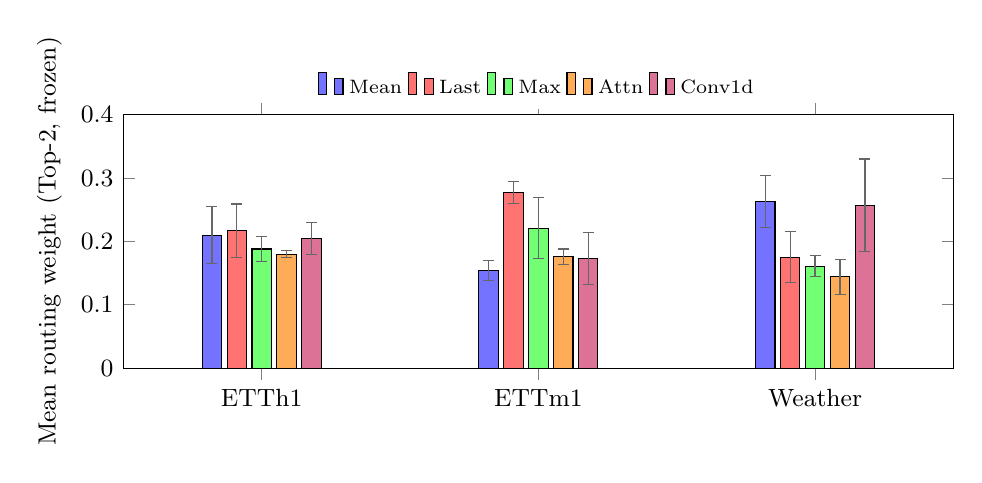
\begin{tikzpicture}
\begin{axis}[
    ybar,
    width=\columnwidth,
    height=4.8cm,
    bar width=7pt,
    ylabel={Mean routing weight (Top-2, frozen)},
    ylabel style={font=\small},
    symbolic x coords={ETTh1, ETTm1, Weather},
    xtick=data,
    x tick label style={font=\small},
    y tick label style={font=\small},
    legend style={at={(0.5,1.02)}, anchor=south, legend columns=5, font=\scriptsize, draw=none},
    ymin=0, ymax=0.40,
    enlarge x limits=0.25,
    error bars/y dir=both,
    error bars/y explicit,
    error bars/error bar style={line width=0.5pt, black!60},
]
\addplot[fill=blue!55]   coordinates {(ETTh1,0.210) +- (0,0.045) (ETTm1,0.154) +- (0,0.016) (Weather,0.263) +- (0,0.041)};
\addplot[fill=red!55]    coordinates {(ETTh1,0.217) +- (0,0.042) (ETTm1,0.277) +- (0,0.017) (Weather,0.175) +- (0,0.040)};
\addplot[fill=green!55]  coordinates {(ETTh1,0.188) +- (0,0.020) (ETTm1,0.221) +- (0,0.048) (Weather,0.161) +- (0,0.017)};
\addplot[fill=orange!65] coordinates {(ETTh1,0.180) +- (0,0.006) (ETTm1,0.176) +- (0,0.012) (Weather,0.144) +- (0,0.028)};
\addplot[fill=purple!55] coordinates {(ETTh1,0.205) +- (0,0.025) (ETTm1,0.173) +- (0,0.041) (Weather,0.257) +- (0,0.073)};
\legend{Mean, Last, Max, Attn, Conv1d}
\end{axis}
\end{tikzpicture}
\caption{\textbf{Multi-seed RR-MoA routing weights per dataset} (Top-2 sparse, strictly frozen, mean$\pm$std over seeds $\{42,43,44\}$). Routing is diverse and dataset-dependent: ETTh1 spreads weight roughly uniformly (entropy $1.495\pm0.034$); ETTm1 concentrates on Last+Max; Weather on Mean+Conv1d.}
\label{fig:routing_appendix}
\end{figure}

\section{Extended RR-MoA Freeze Grid}
\label{app:extended_rrmoa}

\begin{table}[h]
\centering
\caption{\textbf{Extended freeze-level ablation} (ETTh2, ETTm2, Electricity; test MSE, mean$\pm$std, 3 seeds, H=96). Continues Table~\ref{tab:rrmoa} from the main text.}
\label{tab:rrmoa_extended}
\small
\begin{tabular}{@{}llccc@{}}
\toprule
Dataset & Freeze level & RR-MoA (Top-2) & Best fixed & $\Delta$\% \\
\midrule
\multirow{3}{*}{ETTh2}
 & Frozen (0/8)   & $\mathbf{0.788 \pm 0.096}$ & $2.748 \pm 0.201$ & $\mathbf{-71.3\%}$ \\
 & Last-2 (2/8)   & $\mathbf{1.302 \pm 0.134}$ & $2.599 \pm 0.085$ & $-49.9\%$ \\
 & Last-4 (4/8)   & $\mathbf{1.745 \pm 0.187}$ & $2.540 \pm 0.110$ & $-31.3\%$ \\
\midrule
\multirow{3}{*}{ETTm2}
 & Frozen (0/8)   & $\mathbf{0.588 \pm 0.021}$ & $2.556 \pm 0.028$ & $\mathbf{-77.0\%}$ \\
 & Last-2 (2/8)   & $\mathbf{0.867 \pm 0.083}$ & $2.915 \pm 0.202$ & $-70.3\%$ \\
 & Last-4 (4/8)   & $\mathbf{0.731 \pm 0.157}$ & $2.740 \pm 0.092$ & $-73.3\%$ \\
\midrule
\multirow{3}{*}{Electricity}
 & Frozen (0/8)   & $\mathbf{0.386 \pm 0.059}$ & $0.525 \pm 0.026$ & $-26.4\%$ \\
 & Last-2 (2/8)   & $\mathbf{0.336 \pm 0.023}$ & $0.482 \pm 0.005$ & $\mathbf{-30.3\%}$ \\
 & Last-4 (4/8)   & $\mathbf{0.344 \pm 0.021}$ & $0.472 \pm 0.023$ & $-27.2\%$ \\
\midrule
\multicolumn{3}{l}{\textbf{Combined with Table~\ref{tab:rrmoa}: RR-MoA wins}} & \multicolumn{2}{c}{\textbf{54/54 (100\%)}} \\
\bottomrule
\end{tabular}
\end{table}

\begin{table}[h]
\centering
\caption{\textbf{Extended AdaMix routing collapse} (ETTh2, ETTm2, Electricity). Continues Table~\ref{tab:adamix} from the main text.}
\label{tab:adamix_extended}
\small
\begin{tabular}{@{}llcc@{}}
\toprule
Dataset & Freeze level & MSE (mean$\pm$std) & Routing entropy (mean$\pm$std) \\
\midrule
\multirow{3}{*}{ETTh2}
 & Frozen  & $2.625 \pm 0.219$ & $0.636 \pm 0.385$ \\
 & Last-2  & $2.985 \pm 0.024$ & $0.353 \pm 0.499$ \\
 & Last-4  & $2.885 \pm 0.150$ & $0.541 \pm 0.648$ \\
\midrule
\multirow{3}{*}{ETTm2}
 & Frozen  & $2.946 \pm 0.076$ & $0.316 \pm 0.342$ \\
 & Last-2  & $3.114 \pm 0.004$ & $\mathbf{0.000 \pm 0.000}$ \\
 & Last-4  & $2.997 \pm 0.162$ & $0.505 \pm 0.714$ \\
\midrule
\multirow{3}{*}{Electricity}
 & Frozen  & $0.625 \pm 0.220$ & $1.003 \pm 0.315$ \\
 & Last-2  & $1.055 \pm 0.000$ & $\mathbf{0.000 \pm 0.000}$ \\
 & Last-4  & $1.055 \pm 0.001$ & $0.001 \pm 0.002$ \\
\bottomrule
\end{tabular}
\end{table}

\section{Factorial Decomposition}
\label{app:decomposition}

We decompose the contributions of three factors across 6 evaluation datasets: (1) search space representation (code vs.\ discrete), (2) evolutionary selection pressure, and (3) LLM guidance.

\textbf{Code space $\gg$ discrete space.} All code-space methods outperform discrete evolutionary search (Evo-3epoch, 144 distinct adapter graphs) on 6/6 datasets (Wilcoxon signed-rank $p{=}0.031$, Cohen's $d{=}0.82$). The search space representation is the dominant factor.

\textbf{LLM patterns are individually superior.} Within AAS runs, adapters containing LLM-discovered patterns achieve 19.6\% lower MSE than basic architectures ($p{=}0.003$, Mann-Whitney $U$, $n{=}90$, Cohen's $d{=}0.67$). LLM adapters also use 38\% fewer parameters (mean 110K vs.\ 177K).

\textbf{Validity determines aggregate winner.} The LLM wastes 25\% of evaluations on invalid code; templates achieve 100\% validity.

\textbf{Search budget sufficiency.} We tested 14 budget configurations (20--480 evaluations) across ETTh1 and ETTm1; all beat the conv baseline, even at $B{=}20$ (Appendix~\ref{app:budget}). The curve plateaus around $B\!\approx\!60$.

\section{Top-$k$ Sparse Routing Ablation}
\label{app:topk}

\begin{table}[h]
\centering
\caption{\textbf{Top-$k$ sparse routing ablation on ETTh1 (last-2 freeze, 3 seeds).} Top-2 is the operating point used throughout the paper.}
\label{tab:topk}
\small
\begin{tabular}{@{}lcccc@{}}
\toprule
Sparsity ($k$) & Active experts & Active expert FLOPs & Test MSE & $\Delta$ vs Dense \\
\midrule
$k{=}1$ & 1/5 & 20\% & $1.268 \pm 0.072$ & $+130\%$ \\
$k{=}2$ (default) & 2/5 & 40\% & $\mathbf{0.727 \pm 0.074}$ & $+32\%$ \\
$k{=}3$ & 3/5 & 60\% & $0.679 \pm 0.042$ & $+23\%$ \\
Dense $k{=}K{=}5$ & 5/5 & 100\% & $0.550 \pm 0.029$ & --- \\
\bottomrule
\end{tabular}
\end{table}

\textbf{Compute overhead.} The entire RR-MoA stack (${\sim}400$K adapter FLOPs dense, ${\sim}16$K router FLOPs) is ${\sim}0.003\%$ of a MOMENT-small forward pass (${\sim}15$ GFLOPs) and ${\sim}0.001\%$ for Top-2. On MOMENT-large the ratio drops below $0.0002\%$.

\section{Imputation Results}
\label{app:imputation}

\begin{table}[h]
\centering
\caption{Imputation task (20\% masked reconstruction, test MSE, seed 42). RR-MoA wins 3/3.}
\label{tab:imputation}
\small
\begin{tabular}{@{}lccccc@{}}
\toprule
Dataset & Linear & Dense MLP & Conv & Attn & \textbf{RR-MoA} \\
\midrule
ETTh1 & 0.242 & 0.339 & 0.254 & --- & \textbf{0.138} (--43\%) \\
ETTm1 & --- & 0.218 & --- & --- & \textbf{0.104} (--52\%) \\
Weather & --- & 0.195 & --- & --- & \textbf{0.061} (--69\%) \\
\bottomrule
\end{tabular}
\end{table}

\section{DLinear Calibration}
\label{app:dlinear}

\begin{table}[h]
\centering
\caption{\textbf{DLinear supervised calibration} (trained from scratch, no backbone, 3 seeds, test MSE mean$\pm$std). The gap to RR-MoA is expected; the frozen-backbone paradigm is motivated by deployment constraints (\S\ref{sec:intro}).}
\label{tab:dlinear}
\small
\begin{tabular}{@{}lccc@{}}
\toprule
Dataset & DLinear (from scratch) & RR-MoA (frozen, Top-2) & Gap \\
\midrule
ETTh1   & $0.416 \pm 0.002$ & $0.690 \pm 0.021$ & $+65.9\%$ \\
ETTm1   & $0.322 \pm 0.004$ & $0.572 \pm 0.073$ & $+77.6\%$ \\
Weather & $0.208 \pm 0.003$ & $0.289 \pm 0.008$ & $+38.9\%$ \\
\bottomrule
\end{tabular}
\end{table}

\section{Deployment-Regime Motivation}
\label{app:deployment}

The frozen-backbone paradigm is motivated by three deployment regimes where full fine-tuning is infeasible:

\textbf{(i) Multi-tenant cloud serving.} A single TSFM sits in GPU VRAM and serves thousands of tenants via lightweight, hot-swappable per-tenant adapters in host RAM. Retraining a separate DLinear per tenant does not amortize the backbone cost and forfeits zero-shot transfer.

\textbf{(ii) On-device and edge deployment.} One backbone is shipped with the device image; per-site adapters are updated over low-bandwidth links. Collecting each site's training data centrally is often impossible for privacy or latency reasons.

\textbf{(iii) Cross-task reuse.} The same frozen backbone drives forecasting, imputation, and classification via different expert pools. We demonstrate the first two tasks explicitly in the main text.

\end{document}
